\documentclass[degree=doctor,bibtype=numeric]{tongjithesis}
\usepackage{tongjiutils}
\usepackage{algorithm}
\usepackage{algpseudocode}
\usepackage{amsmath}
\renewcommand{\algorithmicrequire}{ \textbf{Input:}}  
\renewcommand{\algorithmicensure}{ \textbf{Output:}} 
%参考文献更新使用biblatex包, 使用gb7714-2015标准, 具体参数设置可在cls文件中搜索biblatex进行了解
%加入bib文件(老版本文件依然能够使用)
\addbibresource{ref/refs_from_zotero.bib}   %
\hypersetup{hidelinks}

\begin{document}

% 定义所有的eps文件在 figures 子目录下
\graphicspath{{figures/}}


%%% 封面部分
\frontmatter
\tongjisetup{
  %******************************
  % 注意:
  %   1. 配置里面不要出现空行
  %   2. 不需要的配置信息可以删除
  %******************************
  %
  %=====
  % 秘级
  %=====
  secretlevel={保密},
  secretyear={2},
  % doctor={0}
  %
  %=========
  % 中文信息
  %=========
  % 题目过长可以换行(推荐手动加入换行符,这样就可以控制换行的地方啦)。
  ctitle={蛋白质复合物筛选模型研究},
  cheadingtitle={蛋白质复合物筛选模型研究},    %用于页眉的标题,不要换行
  %cauthor={高盼},
  %studentnumber={1830801},
  cmajorfirst={工学},
  cmajorsecond={计算机科学与技术},
  cdepartment={电子与信息工程学院},
  %csupervisor={关佶红 教授},
  % 如果没有副指导老师或者校外指导老师,把{}中内容留空即可,或者直接注释掉。
  % cassosupervisor={裴刚 教授~(校外)}, % 副指导老师
  % 日期自动使用当前时间,若需手动指定,按如下方式修改:
  % cdate={\zhdigits{2018}年\zhnumber{11}月},
  % 没有基金的话就注释掉吧。
  cfunds={(国家自然基金项目(某项目)资助},
  %
  %=========
  % 英文信息
  %=========
  etitle={Study on protein complex screening model},
  %eauthor={Pan Gao},
  emajorfirst={Engineering},
  emajorsecond={Computer Science and Technology},
  edepartment={School of Electronic and Information Engineering},
  % 日期自动使用当前时间,若需手动指定,按如下方式修改:
  % edate={November,\ 2018},
  % efunds={(Supported by the Natural Science Foundation of China(No.61772367,U1936205))},    
  %esupervisor={Prof. JiHong Guan}
  % eassosupervisor={Prof. Gang Pei (XiaoWai)}
  % }
}
% 定义中英文摘要和关键字
\begin{cabstract}
  蛋白质复合物是蛋白质相互结合完成某一项生物功能的集合。生物学上蛋白质复合物的识别与研究对细胞组成分析、药物预测等至关重要。生物实验的方法可以识别蛋白质复合物,但其成本较高、周期较长,无法满足大规模数据时代的研究需求。
  现有的蛋白质复合物预测算法主要是基于计算的算法,将蛋白质之间广泛的相互作用抽象成图,蛋白质复合物抽象为图中的局部结构,此时蛋白质复合物预测问题转换为局部子图发现问题。复合物预测算法可以从互作网络中挖掘出大量的局部子图样本,但是由于预测算法本身的局限性,预测结果中会存在部分不符合复合物形成规律的样本。基于计算的复合物预测算法不具有对其预测结果的评价能力,无法识别并剔除这部分样本。

  为了识别和剔除这部分对预测结果具有干扰性的样本,本文提出了蛋白质复合物筛选模型,构建了融合结点特征和邻边特征的蛋白质相互作用网络,并进一步构造了复合物特征子图样本集。本文提出了多种复合物筛选模型并针对每个模型进行了模型训练以及复合物筛选验证,复合物筛选模型包括基于图卷积的模型、基于邻边卷积的模型和基于点边消息传递网络的模型。

  本文的研究工作及贡献:

  1)融合结点特征和邻边特征的蛋白质相互作用网络(简称特征互作网络)。基于蛋白质互作数据构建了蛋白质相互作用网络,基于图自编码器、深度随机游走等网络嵌入方法为网络添加了结点特征,基于生物学上的多种相似性特征提取方法为网络添加了邻边特征,最终构建出特征互作网络。

  构造了多种类别的蛋白质复合物特征子图样本集。原始蛋白质复合物数据集以蛋白质集合的形式存在,无法满足样本后筛选工作的要求。本文基于特征子图提取方法,在特征互作网络中构建对应蛋白质复合物数据集的特征子图样本集,包括基于邻居相似性融合多个标准集构建的正样本数据集;基于COACH算法构建的中间样本数据集;基于改进的随机算法构建的负样本数据集;基于核心附属结构的复合物预测算法构建的待筛选数据集。

  2)基于图卷积神经网络的复合物筛选模型。从拓扑数据出发,本文提出了基于图卷积神经网络的复合物筛选模型。该模型基于图自编码器和深度随机游走嵌入得到蛋白质全局特征,并依据蛋白质复合物子图的拓扑结构,基于图神经网络对蛋白质全局特征进行深度融合。本文将该模型与无全局特征的模型、基于拓扑统计特征的模型进行了对比与分析,结果表明了融合全局特征的图卷积神经网络方法的有效性。
  
  3)基于邻边卷积的复合物筛选模型。从生物数据出发,针对蛋白质复合物生物数据抽象程度较低的问题,本文提出了基于邻边卷积的复合物筛选模型。该模型在蛋白质互作网络中嵌入了表达蛋白质功能关联的多种相似性数据,作为互作网络邻边特征,并基于邻边卷积的方法将子图拓扑和邻边特征进行融合。实验对比了有无邻边特征情况下的邻边卷积模型,结果显示了带邻边特征的邻边卷积模型的有效性。

  4)基于点边消息传递网络的复合物筛选模型。从特征融合角度出发,本文提出了基于点边消息传递网络的复合物筛选模型。该模型保留了表示全局拓扑特性的结点特征和表示生物功能特性的邻边特征,采用消息传递的更新方法在蛋白质复合物局部拓扑结构中同时更新结点特征和邻边特征,实现了全局拓扑特征与生物功能特征的动态更新和深度融合。结果表明基于点边消息传递网络地复合物筛选模型能更好地挖掘蛋白质复合物的形成规律,在多个实验中其评价指标的提升达到了最优。

\end{cabstract}

\ckeywords{蛋白质复合物预测;图神经网络;蛋白质相互作用网络;子图分类;图嵌入}

\begin{eabstract}
  A protein complex is a collection of proteins that bind to each other to accomplish a biological function. The identification and research of protein complexes in biology are very important for cell composition analysis, drug prediction and so on. The method of biological experiment can identify protein complex, but its cost is high and the cycle is long, which can not meet the research demand of large-scale data age.
  The existing protein complex prediction algorithm is mainly based on the calculation algorithm, abstracting the wide interaction between proteins into a diagram, protein complex abstraction into the local structure of the diagram, at which time the protein complex prediction problem is transformed into a local sub-graph to find the problem. The composite prediction algorithm can extract a large number of local subgraph samples from the mutual network, but due to the limitations of the prediction algorithm itself, there will be some samples in the prediction results that do not conform to the formation law of the compound. The calculation-based compound prediction algorithm does not have the ability to evaluate its prediction results, and cannot identify and reject this part of the sample.

  In order to identify and reject the samples which are disturbing to the prediction results, this paper presents a protein complex screening model, constructs a protein interaction network that combines node features and adjacent features, and further constructs a sample set of composite feature sub-maps. In this paper, a variety of composite filtering models are proposed and model training and composite filtering validation are carried out for each model, including models based on tortogram remnants, models based on adjacent curly volume, and models based on point edge messaging networks.

  The research work and contribution of this paper:

  1) A network of protein interactions (referred to as a network of features) that combines node features with adjacent features. Based on the protein interoperability data, the protein interaction network is constructed, the node characteristics are added to the network based on the network embedding methods such as graph self-encoder and deep random walk, and the adjacent features are added to the network based on various similarity characteristic extraction methods in biology, and the characteristic interoperability network is finally constructed.

  A sample set of sub-maps of protein complex features in various categories is constructed. The original protein complex dataset exists in the form of a protein collection and cannot meet the requirements of post-sample screening. Based on the feature sub-graph extraction method, this paper constructs the characteristic sub-map sample set of the corresponding protein complex data set in the feature interoperability network, including the positive sample data set built on the basis of multiple standard sets of neighbor similarity fusion, the intermediate sample data set based on THECH algorithm, the negative sample data set based on the improved random algorithm, and the pending filtering data set based on the composite prediction algorithm of the core satellite structure.


  2) A composite screening model based on a refride neural network. Based on the topological data, this paper presents a composite screening model based on the refride neural network. The model obtains the global characteristics of proteins based on graph self-encoder and deep random walk embedding, and based on the topology of protein complex subpic, the global characteristics of proteins are deeply fused based on the graph neural network. In this paper, the model is compared and analyzed with the model without global characteristics and based on topological statistical features, and the results show the effectiveness of the topographical neural network method of fusing global features.

  3) A composite filtering model based on neighboring coils. Based on the biological data, in view of the low abstraction of the biological data of protein complexes, this paper puts forward a composite screening model based on the neighboring reftric. The model embeds a variety of similarity data expressing protein function association in the protein interoperability network, as a mutual network neighbor feature, and fuses the subgraph topology and neighbor feature based on the method of neighbor converse. The experiment compares the neighborhood remnoms model with or without neighbor features, and the results show the validity of the neighboring reuter model with neighbor features.

  4)A composite filtering model based on a point-edge messaging network. From the point of view of feature fusion, this paper proposes a composite filtering model based on point-edge messaging network. The model retains the node characteristics representing the global topological characteristics and the neighbor characteristics representing the biological functional characteristics, and uses the method of message delivery to update the node features and adjacent features in the local topology of the protein complex at the same time, and realizes the dynamic update and deep fusion of the global topological features and biological functional features. The results show that the formation law of protein complex can be better excavated based on the point-edge message transmission network composite screening model, and the improvement of its evaluation index has reached the optimal level in many experiments.

\end{eabstract}

\ekeywords{Protein complex prediction; graph neural network; protein interaction network; sub-graph classification; graph embedding}

\makecover


% 目录
\tableofcontents
% 符号对照表
\begin{denotation}
    \item[GNU] GNU's Not Unix /'gnu:/
\item[GFDL] GNU Free Documentation License
\item[GPL] GNU General Public License
\item[FSF] Free Software Foundation
\item[SMP] 对称多处理
\item[API] 应用程序编程接口
\item[$E$] 能量
\item[$m$] 质量
\item[$c$] 光速
\item[$P$] 概率
\item[$T$] 时间
\item[$v$] 速度

\end{denotation}

%%% 以下索引按需要选择
% 插图索引
\listoffigures
% 表格索引
\listoftables
% 公式索引
% \listofequations
%%% 正文 
\mainmatter
\chapter{绪论}
\label{chapter:intro}


\section{研究背景}
\label{section:intro:background}

生物信息学是研究生物信息的采集、处理、存储、传播和解释等各方面的学科。
生物信息学可以帮助人类从海量的生物数据中挖掘内部的生理过程规律,从而指导进一步的生物学研究。在规模化实验大力发展和海量数据爆发的如今,如何有效的利用生物数据变得越来越中了。
生物信息学分为三个主要的发展阶段,前基因组时代主要建立了各种生物数据库和序列比较算法、基因组时代进行了大规模的基因测序以及目前所处的后基因组时代。
后基因组时代研究重心以生物数据分析为主,并且挖掘的层次逐渐深入。已经从对基因组直接的结构的研究逐渐转向对基因功能的研究,其中的主要侧重点包括基因组学、转录组学以及蛋白质组学等\cite{helms_principles_2019}。

蛋白质是生物细胞和组织的重要组成部分,是生命体的物质基础,也是遗传信息的直接表达手段,涉及生物体载体、免疫、激素等方方面面。蛋白质分子深度参与了组织的构成与修复、生理功能的调节和能量的供给。
蛋白质组学\cite{schubert_quantitative_2017}是在蛋白质表达层面研究生理生化功能为主的一门学科,目的是揭示蛋白质的基本生命活动规律,其中研究主要关注蛋白质结构、蛋白质丰度、蛋白质修饰以及蛋白质相互作用。

蛋自质在细胞活动中发挥着巨大的作用。但是在多数情况下单个蛋自质无法独立的执行生物功能,只有构成蛋白质复合物,才能有效的参与到细胞活动中\cite{gavin_functional_2002}。因此蛋白质复合物的结构、功能及形成方式的研究就显得尤为重要。图\ref{fig:swr1_complex}是具有染色质重塑功能的酵母SWR1复合物。
\begin{figure}[htbp]
  \centering
  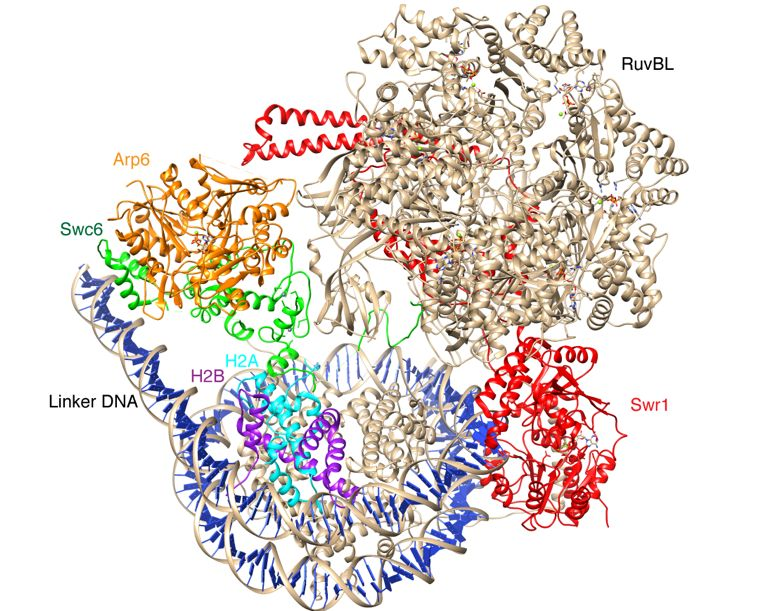
\includegraphics{SWR1_complex}
  \caption{酵母菌SWR1复合物}
  \label{fig:swr1_complex}
\end{figure}
生物实验中检测蛋白质复合物主要通过串联亲和纯化与质谱分析\cite{g_generic_1999}、酵母双杂交\cite{li_identification_1993}两种技术对蛋白质复合物进行分离和鉴定。串联亲和纯化与质谱分析通过靶蛋白标定以及自然条件下亲和纯化获取可能的蛋白质复合物,再使用质谱分析进行鉴定。酵母双杂交技术利用转录调控因子中的组件特征研究蛋白质之间的相互作用关系。虽然基于实验测定的方法具有生物学上的可解释性,但是生物实验往往条件困难、实验步骤多且成本昂贵,无法满足快速增长的研究需求。

蛋白质与生理环境存在广泛的相互作用,蛋白质复杂功能的实现同蛋白质之间、DNA与蛋白质、RNA与蛋白质的相互作用密切相关,蛋白质复合物正是一组强相关的蛋白质组合共同作用的结果。随着生物信息学的发展以及高通量技术的发展,蛋白质相互作用关系(Protein-ProteinInteraction,$PPI$,后简称为互作关系)得到了大量的补充,促成了大规模互作网络的构建\cite{butland_interaction_2005},即蛋白质相互作用网络(Protein-ProteinInteractionNetwork,$PIN$)。图\ref{fig:ppi}为酵母菌蛋白质相互作用网络。
\begin{figure}[htbp]
  \centering
  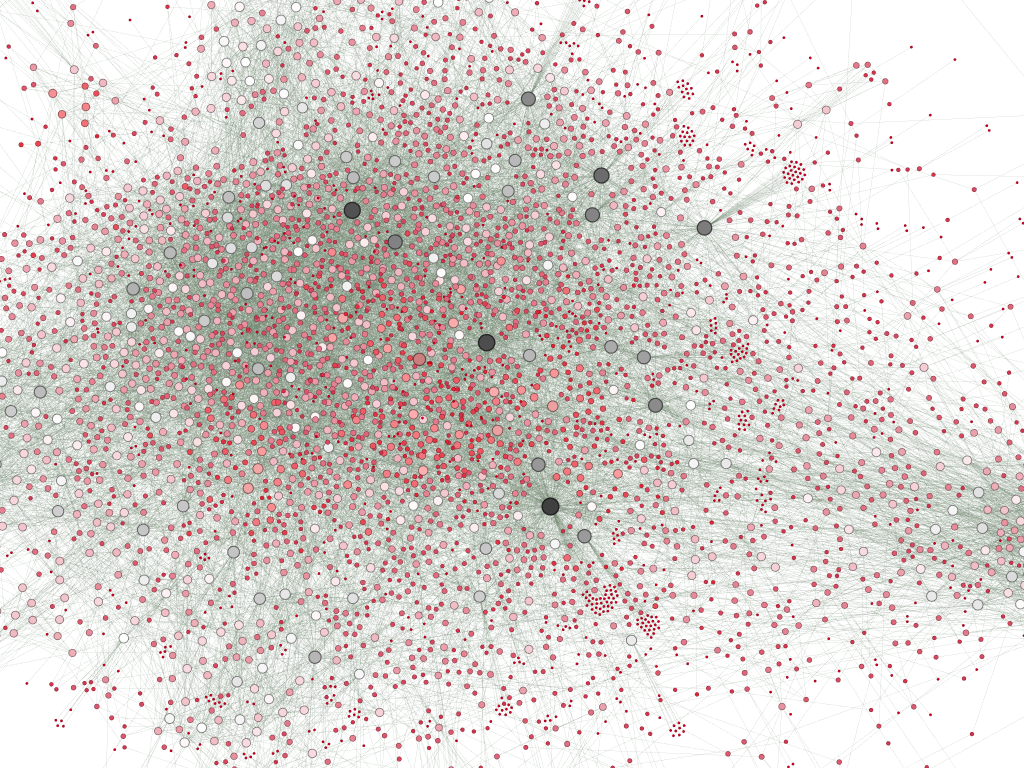
\includegraphics[width=10cm]{ppi-dip-color}
  \caption{酵母菌蛋白质相互作用网络(部分)}
  \label{fig:ppi}
\end{figure}
已知的蛋白质复合物可以视作互作网络里面的一系列子网络,因此利用图论和计算模型学习子网络的分布模式,即可在互作网络中发掘潜在的蛋白质复合物\cite{legrain_proteinprotein_2001}。利用图论的方法,蛋白质互作网络可以转换为无向图~$G=(V,E)$。其中$V$为图中结点的集合,表示所有的蛋白质,$E$为图中邻边的集合,表示所有的蛋白质互作关系。$PIN$转换为图结构之后,图论上的计算模型和深度学习方法就可以迁移到蛋白质复合物的研究中。2002年,Tong\cite{tong_combined_2002}等人提出了密集子图的假说,蛋白质复合物在$PIN$是密集链接的子图,而与其他的蛋白质连接相对稀疏。在$PIN$中预测蛋白质复合物的问题就转换为了密集子图的挖掘问题,逐渐发展出了利用$PIN$和计算方法识别蛋白质复合物的理论。

\section{国内外研究现状}
\label{section:intro:research}

现有的基于计算方法的蛋白质复合物预测方法主要分为五类:基于网络结构的图聚类方法、融合生物信息的图聚类方法、核心附属扩展方法、动态网络方法以及监督学习方法。以下分别对这五类方法的研究现状做简单的介绍。

\subsection{基于网络结构的图聚类方法}
\label{subsection:research:TopologyMethod}

现有大多数复合物预测方法为基于网络结构的图聚类方法,基本思路是在无权无向图中挖掘密集子图。这类方法较为简单明确,取得了一定的成果。

MCODE算法\cite{bader_automated_2003}是最早提出基于网络结构构造密集子图的复合物预测算法。首先算法会计算所有结点的局部邻居密度,其中密度超过平均值的结点成为种子,视作初始子图。满足相应阈值条件的邻居结点不断扩充子图,直到阈值条件饱和,最终子图视为预测的复合物,算法最终会过滤掉结点数少的复合物。
Clique算法\cite{spirin_protein_2003}通过穷举法、超顺磁性聚类和蒙特卡洛模拟三种方法搜索完全图来检测蛋白质复合物。
RNSC算法\cite{king_protein_2004}以随机聚簇最为初始聚簇,按照代价函数逐渐削减聚簇,最终形成蛋白质复合物。
Pereira‐Leal\cite{pereiraleal_detection_2004}提出将马尔科夫聚类算法应用于蛋白质复合物检测,通过转移矩阵的自乘来扩展连通区域,通过幂运算进行膨胀操作只保留生成概率高的区域。膨胀和扩展操作交替运行,收敛之后获得蛋白质复合物。
LCMA算法\cite{li_interaction_2005}从$PIN$中较小的完全图开始,通过不断合并重合率高的完全图来检测蛋白质复合物。CFinder算法\cite{adamcsek_cfinder_2006}进一步定义了搜索与合并的策略,算法首先寻找网络中的k阶完全图,如果两个子图之间有k-1个公共结点,则定义为两个k阶完全图相邻,将两个子图合并。算法通过不断合并k阶完全图预测蛋白质复合物。
SCAN算法\cite{mete_structural_2008}认为一对蛋白质的公共邻居超过阈值时,这对蛋白质可被视为结构可达,可以作为种子蛋白质继续扩展其余结构可达蛋白质。
ClusterONE算法\cite{nepusz_detecting_2012}充分利用了蛋白质复合物内部连接密集,外部连接稀疏的假设,并且明确定义了子图紧密性。其主要思路是首先按照结点度排序获取种子结点,种子结点向外扩展操过程中可以添加或删除结点,以达到局部子图最佳紧密性。
Zheng等人\cite{zheng_protein_2020}进一步改进了图紧密性定义,提出根据子图中3阶完全图个数来定义局部子图连紧密性。

有部分研究将$PIN$中的结点做预分类以达到更优的结果。
CPridict算法\cite{xu_function_2014}首先计算蛋白质之间的功能相似性,然后$PIN$以功能相似性做谱聚类,将蛋白质分为多个分组,各个分组独立进行复合物预测。CPridict2.0算法\cite{xu_effective_2017}进一步基于FunCat功能目录对蛋白质进行分组。
CODEC算法\cite{geva_identification_2011}基于质谱实验将蛋白质分类为诱饵蛋白和靶标蛋白,从靶标蛋白及其邻居结点开始,通过增减结点获得最大子图得分。

\subsection{网络预处理的图聚类方法}
\label{subsection:research:appendBiology}
蛋白质复合物的预测是一个复杂的生物学问题,而由于实验手段的限制,互作数据存在着高假阴性和高假阳性的缺陷\cite{von_mering_comparative_2002}。研究者开始尝试挖掘网络拓扑特征,对网络结构进行修复和连边加权处理,提高$PIN$的可信度以获取更精确的聚类结果。
DPClus算法\cite{altaf-ul-amin_development_2006}最早对$PIN$做加权处理,根据一对结点公共邻居数量给这对结点之间的边加权,结点的权重所有邻边的权重之和。权重较大的结点作为种子结点,通过紧密型结点的连接预测蛋白质复合物。
PCP算法\cite{chua_using_2008}利用使用FS-weight计算邻边的可靠度,并移除网络中可靠度较低的边,之后利用完全图发现合并算法检测复合物。
CMC算法\cite{liu_complex_2009}采用了一种迭代式的边加权方法,不断的以结点的加权公共邻居数更新邻边权重,完全图评价分数也和子图的权重有关。
Bootstrap算法\cite{friedel_bootstrapping_2009}基于boostrap采样法预测复合物,在网络中做有放回重复采样,多次采样确定蛋白质相互作用权重,再进行多次执行马尔可夫聚类算法,形成蛋白质聚簇。最终以蛋白质在聚簇网络中的贡献性重构$PIN$权重。

除了基于拓扑结构的加权方法,还可以利用生物信息对相互作用加权。已有研究表明\cite{komurov_revealing_2007},形成功能团的蛋白质通常具有相同的基因表达。部分研究借助基因表达数据更改权重,重新定义密集子图的评价函数以达到更优的聚类效果。
MATISSE算法\cite{ulitsky_identification_2007}使用基因表达数据的相关性衡量蛋白质的互作强度,并以此定义$PIN$的权重,再将聚类算法运用到加权网络预测蛋白质复合物。
GFA算法\cite{jianxing_feng_max-flow-based_2011}基于最密子图算法获取互作网络中的最密子图,将子图的密度定义为子图内基因表达量之和,在聚类结果中选取密度较大的子图为复合物。

蛋白质复合物中,蛋白质的功能表达往往趋向于相近或者相同,因此功能表达数据也有助于蛋白质相互作用加权。Lubovac等人\cite{lubovac_combining_2006}在基因本体信息\cite{ashburner_gene_2000}(GENE Ontology,简称GO)形成的有向无环图上,使用SWEMODE算法计算两个蛋白质的功能相似性。在$PIN$中结点权重通过聚合邻边权重以及邻居数计算,后续借鉴MCODE在结点和邻边均加权的网络中预测蛋白质复合物。WCOACH算法\cite{kouhsar_wcoach_2016}同样使用蛋白质功能表达数据加权,在加权网络上运用改进的COACH算法\cite{leung_predicting_2009}。

有研究表明,蛋白质结构域互作信息也会对蛋白质复合物的形成产生影响\cite{kim_relating_2006},多对蛋白质无法作用于互作界面的重复区域。Jung等人\cite{jung_protein_2008}利用这个特性,剔除了MCODE和LCMA生成的结果中具有结构域冲突的复合物,提高了结果的准确性。DACO算法\cite{will_identifying_2014}将蛋白质相互作用和结构域相互作用数据结合起来,使用图聚类算法预测蛋白质复合物时,进行结构域的紧密优化,预测出来的复合物确保存在结构域互作的可能性。


\subsection{核心附属扩展方法}
\label{subsection:research:CoreAppend}

SCAN算法\cite{mete_structural_2008}已经提出了基于种子蛋白质扩展的复合物预测方法。然而种子蛋白质仅仅时拓扑结构上的聚类核心,并不具有明显的生物学意义。研究人员\cite{gavin_proteome_2006}通过酵母菌中复合物的结构发现,部分蛋白质存在于多种复合物中,且这些蛋白质之间存在大量的相互作用关系,组成了复合物的功能单元,此类蛋白质被称为核心蛋白质。在一个复合物中其余蛋白质附着于核心蛋白质,被称为附属蛋白质。如图\ref{fig:core_append}所示,其中深色椭圆形底框部分为复合物中的核心模块。

CORE算法\cite{leung_predicting_2009}是基于蛋白质复合物核心附属形成机理提出的算法,通过计算两个蛋白质公共邻居之间互作情况发现核心蛋白质,通过核心蛋白质周围相互作用关系添加附属蛋白质。COACH算法\cite{leung_predicting_2009}根据蛋白质及邻居在$PIN$网络中的重要程度确定核心蛋白质,其中蛋白质结点权重越大,其成为核心蛋白质的可能性越高。

\begin{figure}[htbp]
  \centering
  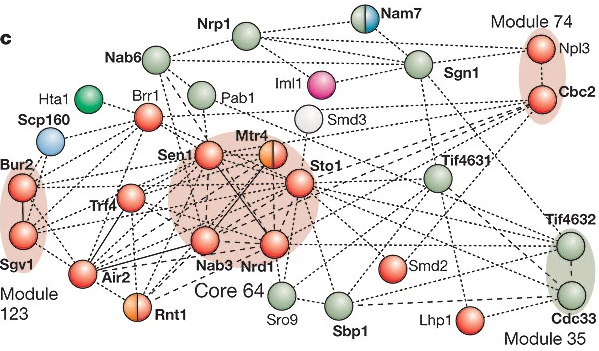
\includegraphics{core_append}
  \caption{核心附属结构示例——Core64部分为核心结构}
  \label{fig:core_append}
\end{figure}

\subsection{监督学习方法}
\label{subsection:research:Supervision}

TODO

\subsection{动态网络方法}
\label{subsection:research:Dynamic}

由于蛋白质会随着生理生化周期不断变化,因此蛋白质相互作用也具有动态特性,部分研究\cite{li_dynamic_2017}将基因表达时序数据和蛋白质相互作用结合,构建动态蛋白质相互作用网络$Dynamic-PIN$。
Tang等人\cite{tang_comparison_2011}设定阈值,将蛋白质基因表达数据超过阈值的蛋白质视为活跃蛋白质,以活跃蛋白质构建动态网络。Ou-Yang等人\cite{ou-yang_detecting_2014}使用基因表达数据区分瞬态和稳态蛋白质。

TODO

\subsection{方法总结}
\label{subsection:research:researchSummary}

表\ref{tab:MethodSummary}给出了现有复合物预测方法的类别、思想以及相关特点。

\begin{table}[h]
  \centering
  \caption{复合物预测方法对照表}
  \label{tab:MethodSummary}
  \begin{tabular}{L{3cm}L{6cm}L{5cm}}
    \toprule
    \textbf{方法类别}          & \textbf{研究思想}                                                              & \textbf{特点}                                                          \\
    \midrule
    局部密集子图的聚类方法     & 挖掘互作网络中的密集子图                                                       & 倾向于预测连接紧密的子图,易受到蛋白质互作假阳性、假阴性的影响         \\\hline
    加权的局部密集子图聚类方法 & 使用多种生物数据对互作网络加权,在加权网络的基础上挖掘密集子图                 & 提高了互作网络可信度,依旧倾向于预测密集子图                           \\\hline
    核心附属结构的预测方法     & 提取核心蛋白质,再在核心蛋白质周围不断添加附属将蛋白质                         & 仅仅针对具有核心附属结构的蛋白质复合物                                 \\\hline
    基于监督学习的方法         & 利用已知复合物辅助的生物、拓扑特征训练分类模型,基于分类模型预测复合物         & 数据融合和模型训练具有一定的难度                                       \\\hline
    动态网络的图聚类方法       & 基于生物数据建立动态蛋白质复合物,再基于动态网络某一时刻的数据预测蛋白质复合物 & 动态网络更贴近生命活动的真实过程,然而预测算法依旧基于密集子图发现算法 \\
    \bottomrule
  \end{tabular}
\end{table}


\section{复合物筛选框架的研究动机和思路}
\label{section:intro:motivationAndThinking}

\subsection{研究动机}
\label{subsection:motivationAndThinking:motivation}
国内外学者对复合物的识别已经提出了诸多方法,总体趋势也是趋向于融合生物数据和网络数据并达到更精确的预测,但是目前现有的方法还存在以下的不足。
\begin{itemize}

  \item 无法充分利用已有的先验知识。上述的研究方法主要是基于无监督方法,在复合物的研究问题上,无监督方法具有训练简单、结构明确的优点。但是随着实验技术更新、生物数据量增加以及图数据挖掘算法的井喷发展,无监督学习方法无法利用已有的先验知识,其预测准确率无法得到进一步提升。有监督学习方法可以通过学习已有复合物的分布特征,挖掘出特定$PIN$网络中蛋白质复合物的分布规律。目前已有的监督方法如Shi提出的方法\cite{shi_protein_2011}仅仅学习复合物的拓扑特征的映射函数,且映射函数只作用于复合物扩展过程中单个结点的取舍判断,算法尚存在大量的改进空间。

  \item 复合物准确度较低。部分模型方法如RNSC算法\cite{king_protein_2004}、Clique算法\cite{spirin_protein_2003}等等具有很强的随机性,此类方法为了达到较高的复合物召回率,往往倾向于产生过量的候选复合物,导致结果的准确率的降低。预测的复合物中存在大量错误的样本,对后续的生物研究有一定的影响。如何在维持复合物预测召回率的情况下,提高预测的准确度是一个值得研究的问题。

  \item 生物信息在$PIN$中融合度低。在\ref{subsection:research:appendBiology}中提到了融合生物信息的诸多方法,然而这些方法只停留在利用生物信息更改$PIN$邻边权重的层面,不同的生物信息如GO注释、基因表达信息、蛋白质保守性等数据被统一编码到了相互作用的边权重中,这个编码转换过程会丢失原有丰富的生物数据。编码过程仅仅作为$PIN$数据的预处理,生物数据无法动态地参与到复合物预测模型的框架设计中。同时,目前也没有方法将生物信息编码到蛋白质结点中,如何有效的利用结点编码增强复合物的预测质量也是一个亟待解决的问题。
\end{itemize}

针对以上蛋白质复合物预测问题中存在的不足,从蛋白质复合物的预测到对预测结果的评价之间存在改进的空间。不同复合物预测方法可以得到大量的复合物预测结果,由于预测方法存在的缺陷,预测结果中存在部分不符合复合物形成规律的样本,而预测方法无法精确的识别并剔除这部分复合物。因此本文基于预测后的评价与筛选模型研究(简称后筛选)动机设计可行且有效的模型框架。

\subsection{可行性分析}
\label{subsection:motivationAndThinking:cando}

两阶段筛选方法在已有领域的应用。
基于两阶段筛选方法在目标检测领域已经得到了广泛的运用,比如RCNN算法\cite{girshick_rich_2014}。在一张图片中检测目标可以分为两个阶段,第一阶段为获取所有可能的框图,第二阶段为对候选框做筛选与调整。对应到蛋白质相互作用网络中预测蛋白质复合物,也可以做类似的处理,首先获取对应的候选复合物,再利用复合物筛选算法,在候选复合物基础上获得更加精确的预测样本,以达到更优的预测结果。在复合物预测邻域,这种两阶段思想具有一定的可行性。

复合物筛选领域已有的部分筛选方法。
在复合物预测邻域,已有部分研究提出过类似的方法,比如RNSC算法\cite{king_protein_2004}提出了基于设定得分函数筛选预测复合物的思想,论文\cite{yu_predicting_2014}提出了使用复合物拓扑性质对复合物做分类的方法。但是目前已有的复合物筛选方法研究均较为有限,已提出的方法未偏计算统计的方法,尚未有算法将生物信息与复合物的拓扑结构结合起来,无法学习蛋白质复合物深层次特征,且此类方法通常只将筛选部分作为特定模型的补充,而非成体系的研究,无法将筛选模型当成一般性方法应用于复合物筛选邻域。为了改进朴素的基于计算的预测方法,本文提出以GCN为基础的一系列复合物分类模型,将复合物的特征与结构结合起来。

可供筛选的复合物样本。
部分复合物筛选算法,如Clique算法\cite{spirin_protein_2003}、Dpclus算法等,是基于随机种子以及子图扩展的方法。这类方法由于能够广泛的挖掘整个$PPI$网络的所有结点,因此其预测结果能够匹配出多数已知的蛋白质复合物。但是此类方法会过多样本,其中大量的具有随机性的复合物对总体的预测结果具有干扰性。使用复合物筛选模型剔除具有随机性的负样本,可以在保持该类方法高召回率的同时,提高预测结果的准确度。


\subsection{研究思路}
\label{subsection:motivationAndThinking:thinking}

本文提出了一种基于监督学习和融合特征的复合物后筛选模型。
算法的核心思想是利用已有的生物数据,包括$PIN$、生物注释信息、已知复合物等等,将蛋白质复合物结点数据转换为可学习的结构化数据,并为结构化的数据添加标签,通过监督学习的方式构建一个鲁棒性的复合物分类模型。

通过模型设计以及合适的训练过程,模型能够融合蛋白质复合物的多种数据,包括该复合物具有哪些蛋白质、具有哪些邻边关系以及特征等等,较为准确的辨别某一个复合物是否为真实复合物,学习复合物的形成规律。
在此模型训练成功的前提下,将一般性的复合物预测算法,比如DPClus算法\cite{altaf-ul-amin_development_2006}、Clique算法\cite{spirin_protein_2003}等产生的复合物交由分类模型做进一步筛选,即filter过程,剔除其中得分较低的不符合复合物形成规律的样本,保留得分高的样本代替为相应算法预测的最终结果。
由于无效样本的剔除,理论上经过filter的处理,相较于未筛选前的样本,最终预测结果的多项评价指标可以得到提升。

\subsection{筛选框架实现流程}
\label{subsection:motivationAndThinking:flow}

复合物筛选模型框架设计如图\ref{fig:main-flow}所示,主要由四个阶段组成,分别是构建融合结点特征和邻边特征的蛋白质相互作用网络;利用特征互作网络构建复合物子图样本集;基于训练数据集中的子图样本训练图分类模型;基于已训练复合物评价模型筛选复合物及对比。其中重要的阶段为第二阶段和第三阶段。

\begin{figure}[htbp]
  \centering
  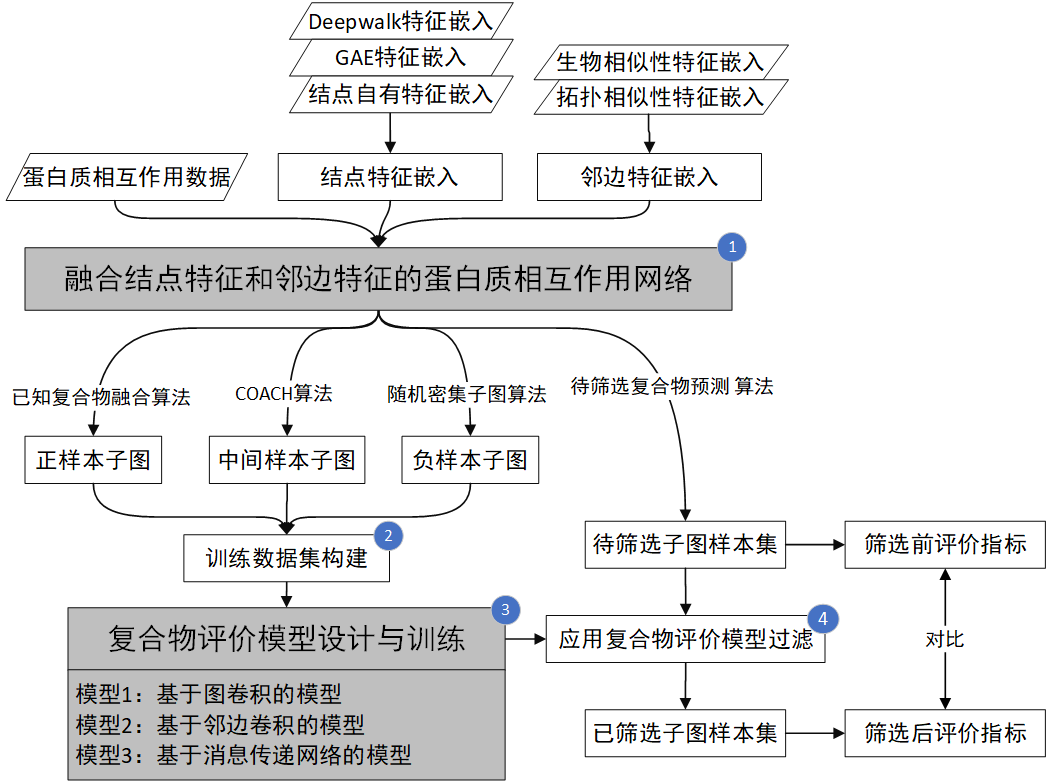
\includegraphics[width=14cm]{main-flow}
  \caption{复合物筛选框架主体流程图}
  \label{fig:main-flow}
\end{figure}

\subparagraph*{第一阶段,构建融合结点特征和邻边特征的蛋白质相互作用网络}

利用蛋白质相互作用数据集构建蛋白质相互作用网络,其中每一个结点代表一个蛋白质,每一条邻边代表蛋白质之间的相互作用关系。然后利用多种结点嵌入方法和邻边嵌入方法给蛋白质相互作用网络添加相应的特征数据。
最终形成特征相互作用网络。
该阶段总体过程如图中标号\textcircled{1}部分所示。

\subparagraph*{第二阶段,利用特征互作网络构建复合物子图样本集}

蛋白质复合物数据集中每一个蛋白质复合物数据都是以蛋白质集合$SET$的形式存在。将$SET$中的蛋白质对应到复合物相互作用网络中的结点集合,在特征互作网络中抽取结点集合对应的子图,得到特征子图数据。

依据复合物数据集来源的不同,特征子图样本可分为已知复合物得到的正样本子图、COACH算法得到的中间样本子图、随机数据得到的负样本子图以及待筛选复合物预测算法得到的待筛选样本子图。
依据已有的复合物评价指标,正样本得分为1、中间样本得分为0~1、负样本得分为0,这些携带标签的样本组合起来作为训练数据集。
该阶段总体过程如图中标号\textcircled{2}部分所示。

\subparagraph*{第三阶段,基于训练数据集中的子图样本训练图分类模型}

训练集中的样本均为图结构数据,每一个图结构数据代表一个蛋白质复合物,且具有结点和邻边特征,同时具有分类标签和评分。在此基础上,基于图分类模型可以训练从特征子图到分类和评分的映射函数,该映射函数作为复合物评价模型。

基于多种图分类模型,本文进行了复合物评价模型的设计与训练。本文涉及了三种图分类模型,分别是以结点卷积的图卷积模型(对应章节\ref{chapter:NodeConv})、以邻边卷积的邻边卷积模型(对应章节\ref{chapter:EdgeConv})和以结点邻边融合的消息传递网络模型(对应章节\ref{chapter:MPNN})。
该阶段具体过程如图中标号\textcircled{3}所示。


\subparagraph*{第四阶段,基于已训练复合物评价模型筛选复合物及对比}

在蛋白质相互作用网络中预测初始复合物,作为待筛选复合物,复合物包括DPClus算法、clique算法等的预测结果。依据标号\textcircled{3}复合物评价模型的评价结果,有一部分评分较高,其余部分评分较低,保留其中评分搞得复合物样本作为筛选后的结果,筛选过程如图中标号\textcircled{4}部分所示。最后本文使用多种的复合物预测评价指标对筛选前后的总体样本进行综合评价,如图中对比部分所示。

\section{研究工作及成果}
\label{section:intro:workandresult}

本文的主要研究工作是基于特征网络的蛋白质复合物筛选算法。针对现有的复合物预测算法无法利用先验知识,本文提出了基于监督学习的复合物筛选模型;针对复合物预测结果精度低,本文提出了二阶段的筛选方法,并进行对比实验验证筛选之后预测样本的评价指标得到了提高;针对现有预测方法无法动态融合$PIN$拓扑结构与相关的特征数据,本文提出了多种特征融合方法,并在方法间进行了对比实验。

实验结果表明,本文筛选模型能够挖掘复合物深层次的规律。在多个复合物预测方法上,经过筛选模型过滤,预测样本的多项评价指标得到了提升,更加精确的预测结果更具有生物学上的参考意义。

本文的主要研究工作和成果包括:

\subparagraph*{构建含特征$PIN$网络结构}

通过生物学上的多种特征提取方法,以及多种网络嵌入方法,本文得到了兼具结点特征和邻边特征的$PIN$网络结构,最终,$PIN$中每一个蛋白质具有82维特征,每一对蛋白质互作具有12维特征,具体特征分布如下。
\begin{itemize}
  \item 结点特征部分:包括Deeowalk特征、GAE特征、蛋白质长度特征;
  \item 邻边特征部分:包括蛋白质功能注释GO特征、结构域特征、亚细胞定位特征、局部拓扑相似性特征;
\end{itemize}

\subparagraph*{复合物子图数据集构建}

利用多个标准集构建了正样本数据集;基于COACH算法的结果构建中间样本数据集;提出了改进的随机算法构建负样本数据集。在$PIN$中抽取复合物子图作为训练样本,对整体数据集中的样本进行了分类和评分,为后续分类模型训练提供数据基础。

\subparagraph*{复合物分类模型研究}

在具有特征网络的前提下,本文研究了多种融合特征的复合物分类模型,提出了基于结点、基于邻边和融合的模型,具体如下。
\begin{itemize}
  \item 基于结点特征模型:提出了基于结点的GCN方法,融合结点的全局拓扑特征进行复合物预测;
  \item 基于邻边特征模型:提出了基于邻边的GCN方法,将初始的邻边特征转换为结点特征,再基于edge-base的GCN方法对特征进行融合;
  \item 特征融合模型:提出了融合结点特征和邻边特征的MPNN方法,提出了结点特征和邻边特征交替更新的方法,在特征融合同时保留自身关键特征。子图特征分为MPNN得到的可学习特征和基于图论得到的计算统计特征,两部分特征结合具有更好的预测准确度;
\end{itemize}

\subparagraph*{相关对比实验及验证}

本文进行了多项实验验证模型的有效性,在DIP网络和Biogrid网络上进行分别训练了各个预测模型,并在Dpclus、ipca等方法上验证筛选结果,验证的指标包括f1值和复合物预测邻域的融合指标。

\section{论文组织}
\label{section:intro:organization}

本论文分为五大章节,具体如下:

第一章,绪论。

第二章,数据处理。

第三章,复合物筛选模型设计。

第四章,实验结果与分析。

第五章,总结与展望。
\chapter{蛋白质复合物特征子图样本生成}
\label{chapter:featSubNetworkConstruct}

\section{蛋白质相互作用特征网络构建}
\label{section:featSubNetworkConstruct:featPPINetwork}

\subsection{基于互作关系构建蛋白质相互作用网络}
\label{subsection:featPPINetwork:networkConstruct}

酿酒酵母(Saccharomyces cerevisiae)的蛋白质相互作用中有较深入的研究,其标准复合物数据集,蛋白质相互作用数据较为完备,因此本文基于酿酒酵母的蛋白质互作网络展开研究。

本文选取了主流的酿酒酵母细菌的$PPI$数据集,包括DIP\cite{salwinski_database_2004}、Krogan\cite{krogan_global_2006}、Biogrid\cite{stark_biogrid_2006}和Gavin\cite{gavin_proteome_2006}。

DIP数据集是结合各种来源的信息创建的一致的$PPI$数据集,可以自动从论文中提取关系数据并更新数据库,同时有专业人员管理。
Krogan数据集使用$LC_MS/MS$技术检测蛋白质相互作用并借助机器学习方法提高结果的可靠度,数据集分为核心和附属两个部分,本文将核心附属网络融合进行实验。
Biogrid数据集融合了多个数据集来源,同时排出了不符合多重验证标准的相互作用。
Gavin数据集基于亲和纯化与质谱技术检测蛋白质相互作用,并使用socio-affinity指数评估$PPI$检测结果的可靠度。

每个数据集都由若干蛋白质相互作用对组成,表示两个蛋白质之间存在相互作用关系,依据关系数据,可以相应的构造$PIN$。数据集具体的网络结构如图\ref{fig:ppi-datasets}所示,具体统计学特征如表\ref{tab:PPIStatic}所示。

\begin{figure}[htbp]
    \centering
    \subcaptionbox{DIP数据集}{\label{fig:ppi:zitu:a}
        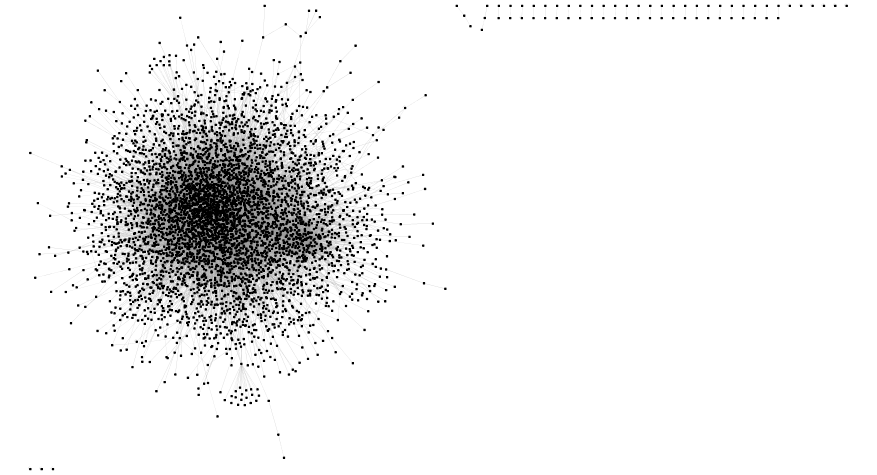
\includegraphics[width=9cm]{ppi-dip}}
    \vskip0.5cm
    \subcaptionbox{Krogan数据集}{\label{fig:ppi:zitu:b}
        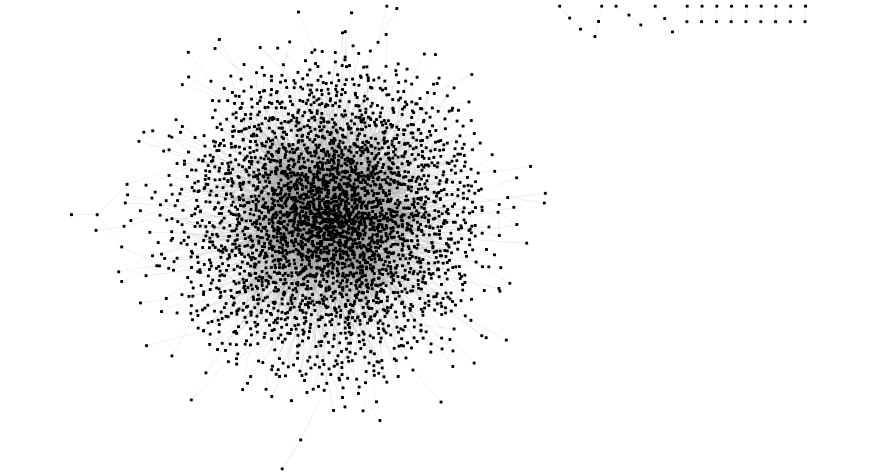
\includegraphics[width=9cm]{ppi-krogan}}
    \vskip0.5cm
    \subcaptionbox{biogrid数据集}{\label{fig:ppi:zitu:c}
        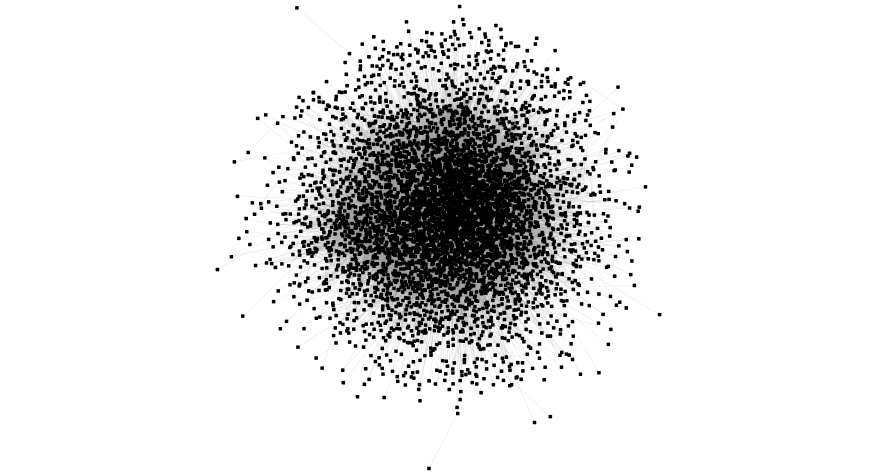
\includegraphics[width=9cm]{ppi-biogrid}}
    \vskip0.5cm
    \subcaptionbox{Gavin数据集}{\label{fig:ppi:zitu:d}
        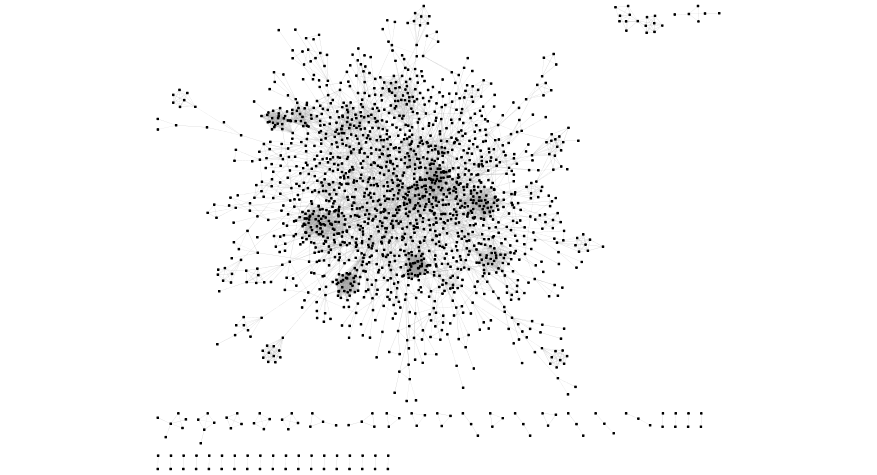
\includegraphics[width=9cm]{ppi-gavin}}
    \caption{蛋白质相互作用数据集}
    \label{fig:ppi-datasets}
\end{figure}


\begin{table}[h]
    \centering
    \caption{$PPI$数据集统计表}
    \label{tab:PPIStatic}
    \begin{tabular}{L{4.2cm}L{2cm}L{2cm}L{2cm}L{2cm}}
        \toprule
        \textbf{网络特征} & \textbf{DIP} & \textbf{Krogan} & \textbf{Biogrid} & \textbf{Gavin} \\
        \midrule
        蛋白质数          & 4928         & 3672            & 5573             & 1855           \\
        相互作用数        & 17201        & 14317           & 59636            & 7669           \\
        平均度数          & 6.98         & 7.80            & 21.40            & 8.27           \\
        密度              & 0.0014       & 0.0021          & 0.0038           & 0.0044         \\
        平均聚类系数      & 0.0945       & 0.1203          & 0.2483           & 0.4674         \\
        连通个数          & 28           & 14              & 1                & 43             \\
        最大连通结点数    & 4873         & 3642            & 5573             & 1727           \\
        传递性            & 0.0728       & 0.1001          & 0.0657           & 0.5676         \\
        直径              & 11           & 10              & 6                & 13             \\
        \bottomrule
    \end{tabular}
\end{table}

从表\ref{tab:PPIStatic}中可以看出,DIP数据集和Biogrid数据集是结点数和邻边数最大的两个数据集,同时其度数差异性较大,本文的研究工作主要围绕这两个数据集展开。最后,本文得出的模型效果也会在Krogan数据集和Gavin数据集进行验证。

利用$PPI$数据集构建相应的$PIN$网络结构之后,可以将蛋白质特征以及蛋白质相互作用特征添加到网络中去,形成带有生物特征的蛋白质相互作用网络$Feated-PIN$。在蛋白质相互作用网络结点上添加蛋白质自有特征和嵌入特征作为结点的初始特征。蛋白质自有特征包括蛋白质序列长度、分子重量特征,蛋白质嵌入特征包括图自编码器器(Graph Auto Encoding,简称GAE)和结点嵌入模型(Node2Vec)得到的图嵌入特征。在蛋白质相互作用网络邻边上添加通过生物计算的蛋白质相互作用特征,包括蛋白质功能注释特征、拓扑域相似性特征和亚细胞定位相似性特征,以及蛋白质拓扑域相似性特征作为图网络里面邻边的初始特征。

\subsection{基于GAE和Deepwalk的结点特征嵌入}
\label{subsection:featPPINetwork:nodeFeatConstruct}

\subsubsection{基于图自编码器的结点特征嵌入}





GAE基于蛋白质复合物网络的编码与解码实现。蛋白质分子的初始特征为随机特征,编码过程采用2层GCN网络,得到蛋白质分子的隐层表示,解码过程通过结点隐层表示预测结点之间的连接强度,恢复网络拓扑结构。损失函数为预测的$PIN$邻接矩阵和真实邻接矩阵的MSELoss(Mean Square Error Loss)。本文得到的GAE产生的结点特征维度为16维。
\subsubsection{基于Deepwalk的结点特征嵌入}



Deepwalk基于蛋白质为源点在$PIN$网络中随机游走,得到随机游走序列,该序列为图中结点与结点共现关系的描述。通过Word2Vec的方式,获取序列中每一个结点的向量表示。本文得到的Deepwalk产生的结点特征维度为64维。
\subsubsection{基于蛋白质自有特征的结点特征嵌入}

\subsubsection{结点特征嵌入汇总}

\subsection{基于多种相似性计算方法的邻边特征嵌入}
\label{subsection:featPPINetwork:edgeFeatConstruct}


\subsubsection{蛋白质GO功能注释相似性的邻边特征嵌入}

基因本体信息\cite{ashburner_gene_2000}即GO注释信息是描述蛋白质功能表达的词汇表,将生物活动过程进行统一编码表示,其在生物信息学邻域得到了广泛的应用。对应到蛋白质中,蛋白质分子参与的若干生物过程均可对应到GO注释表,形成对该蛋白质的综合功能描述。GO注释项总体分为三类,分别是生物过程(Biological Process)、分子功能(Molecular Function)及细胞组成(Cellular Component),生物过程描述分子功能有序组成的生命活动,分子功能描述分子在生物学上的活性,细胞组成描述了亚细胞结构及位置信息。GO注释项之间由于描述涵盖范围的不同,具有一定的从属关系,所有的GO注释项可以组成有向无环图(Directed Acyclic Graph,简称DAG)。图\ref{fig:go-dag}为QuickGO\cite{binns_quickgo_2009}网站中获取的生殖细胞发育过程对应的GO注释DAG图。GO注释信息的从属关系主要分为两种,分别是$is\_a$和$part\_of$,其中$is\_a$表示包含关系,如图中黑色箭头所示,$part\_of$表示从属关系,如图中蓝色箭头所示。图中每一个方框展示了GO注释项及其生物功能。
\begin{figure}[htbp]
    \centering
    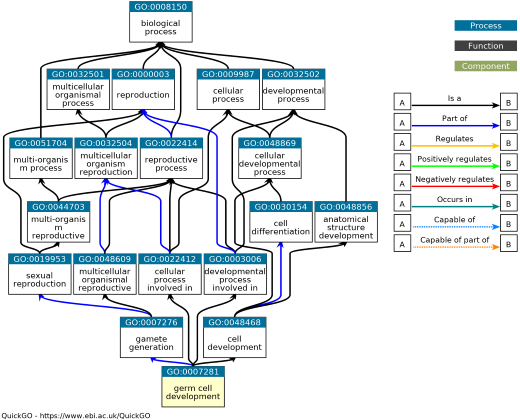
\includegraphics{go-dag}
    \caption{生殖细胞发育对应的GO示意图}
    \label{fig:go-dag}
\end{figure}

通常情况下,蛋白质复合物中蛋白质倾向于相同的功能表达,同时功能表达相似性越高时,蛋白质产生相互作用的可能性越大。部分算法\cite{ulitsky_identification_2007,jianxing_feng_max-flow-based_2011}基于功能表达数据提出了$PIN$连边权重更新的方法。
本文采用两种方法计算蛋白质功能相似度,将计算结果作为$PIN$网络中邻边的蛋白质功能特征。

\paragraph*{基于DAG图的GO相似性计算}

本方法参考了Wang等人\cite{wang_new_2007}提出的方法,给定一个GO注释项$p$,从GO的总体DAG图中提取子图$DAG_p(A,T_p,E_p)$,其中$T_p$是$p$及所有$p$的祖先结点的注释项,$E_p$表示所有截取的注释项的连接关系。
定义$T_p$中每一个结点对$p$的语义值如下:
\begin{equation}
    \label{equ:feat:go:SAT}
    S_p(t)=\left\{\begin{array}{l}
        1,t=p                                                                        \\
        \max {\{ w_e\times S_p(t^\prime )| t^\prime\in ~children~of~(t) \} },t\neq p \\
    \end{array}\right.
\end{equation}
其中$w_e$是$t^\prime$和$t$之间的权重,定义两种类型的边$is\_a$和$part\_of$权重各自为0.8和0.6。有公式可以直观得出,祖先结点点中离$p$注释越远的注释项,其对$p$的语义值越小,而$p$对自身的语义值贡献为1。
定义了所有祖先结点对$p$的语义值之后,可以直接得出$p$的语义值得分,计算公式如下:
\begin{equation}
    \label{equ:feat:go:SVA}
    SV(p)=\sum_{t \in T_p}(t)
\end{equation}
按照该计算方法,可以得到每一个注释项各自的语义值,在此基础上可以得到两个注释项$p$,$q$语义值的相似度,具体计算方法如下:
\begin{equation}
    \label{equ:feat:go:SimItemWang}
    WSim_{GO}(p,q)=\frac{\sum_{t \in T_p \cap T_q}(S_p(t)+S_q(t))}{SV(p)+SV(q)}
\end{equation}
其中$t$为$p$和$q$的所有公共祖先结点。由于蛋白质通常是由多个注释项组成,因此蛋白质之间的功能相似性需要考虑两个蛋白质各自注释项之间的综合结果,其具体计算方法如下:
\begin{equation}
    \label{equ:feat:go:SimProteinWang}
    \begin{aligned}
        WSim_{Protein}(P,Q) & =\frac{1}{m+n}\cdot \left\{\sum_{1\leq i\leq m}{\max_{1\leq j\leq n}[{Sim_{GO}(p_i,q_j)}}]\right. \\
                            & \left.+\sum_{1\leq j\leq n}{\max_{1\leq i\leq m}[{Sim_{GO}(p_i,q_j)}}]\right\}
    \end{aligned}
\end{equation}
其中$P$,$Q$表示两个蛋白质,其中分别具有$\{p_i| i=1,2,\dots,m\}$,$\{q_j| j=1,2,\dots,n\}$的功能注释项。
这个方法的核心思想是将两个蛋白质的注释信息相互关系矩阵$m\times n$构造出来,只考虑源蛋白质的某一个注释项和目标蛋白质所有注释项最大的相关性,而蛋白质的相互作用关系是所有最大值的平均。

\paragraph*{基于频率统计的GO相似性计算}

本方法参考了Lin等人\cite{lin_information-theoretic_1998}提出的方法。首先计算某两个注释项之间的相关性,具体计算过程如下:
\begin{equation}
    \label{equ:feat:go:SimItemLin}
    LSim_{GO}(p,q)=\min_{anc \in Ancient(p,q)}\mathcal{P} (anc)
    % Sim_{GO}(p,q)=\max{\frac{2\times \log }{} }
\end{equation}
其中$Ancient(p,q)$表示两个注释项的公共祖先,而$\mathcal{P}$表示某一个注释项在所有蛋白质中出现的概率。这个计算公式直观的认为,两个具有相互关联的功能注释,其关联结点越稀有,则表示两个注释项的相关性越强。计算蛋白质功能相似性的计算方法如下:
\begin{equation}
    \label{equ:feat:go:SimProteinLin}
    LSim_{Protein}(P,Q)=\max{\frac{2\times \log \{Sim_{GO}(p,q)\}}{\log {\mathcal{P}_p}+\log {\mathcal{P}_q}} }
\end{equation}

\subsubsection{蛋白质结构域相似性的邻边特征嵌入}

蛋白质结构域时蛋白质具有独立功能和特异结构的区域,结构域互作信息影响蛋白质复合物的形成\cite{kim_relating_2006}。结构域之间具有相互作用关系,这些相互作用关系可以从三维交互域(3did)数据库\cite{mosca_3did_2014}提取,并构建成结构域相互作用网络(Domain-Domain Interaction Network,简称DDI)。
单个蛋白质所具有的结构域可以映射到结构域互作网络的若干结点,成为一个结构域集群,而蛋白质域相似性可以转换为两个结构域集群的相互作用关系。
本文中两个蛋白质的结构域互作特征包括如下方面:两个蛋白质结构域交集、并集以及相互之间的差集;映射到结构域相互网络之后,两个结构域集群之间的相互作用关系数量,其具体的计算公式如下:
\begin{equation}
    \label{equ:feat:domain}
    Sim_{domain} = \sum_{i \in dom(p)}{\sum_{j \in dom(q)}{Weight_{ij}}}
\end{equation}
其中$i$、$j$分别时蛋白质$p$、$q$之间的结构域,$Weight_{ij}$代表结构域$i$、$j$在结构域相互作用网络中的作用强度,对于无权网络可以取值为1。

huang等人\cite{huang_protein-protein_2013}在运用结构域相互作用网络预测蛋白质相互作用时,提出了使用一阶邻居和二阶邻居计算$domain$相似性的想法,其扩展方式如图\ref{fig:domain-second}所示。本文也同时补充了一阶和二阶扩展之后的蛋白质$domain$相似性特征。
\begin{figure}[htbp]
    \centering
    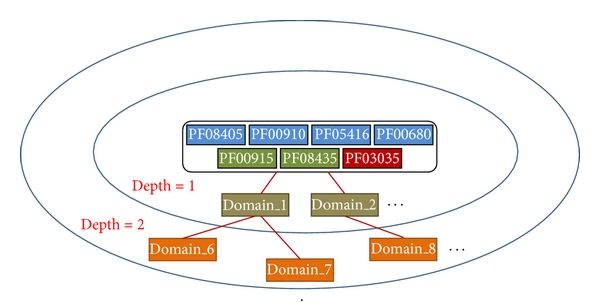
\includegraphics{domain-second}
    \caption{DDI多阶邻居示意图}
    \label{fig:domain-second}
\end{figure}

\subsubsection{蛋白质亚细胞定位相似性的邻边特征嵌入}

细胞是一个高度有序的结构,胞内根据空间分布和功能不同,可以分成不同细胞器或细胞区域,蛋白质只有转运到正确的部位才能参与细胞的各种生命活动,ZHANG等人\cite{zhang_protein_2007}认为蛋白质的亚细胞定位有助于研究蛋白质的生物学功能,同时对蛋白质的其他研究如相互作用、进化等也能提供必要的信息。huang等人提出\cite{fan_genome-wide_2017}使用蛋白质复合物和亚细胞定位信息预测关键蛋白质,蛋白质复合物,蛋白质复合物的生成和功能实现和其所处的细胞位置相关,因此蛋白质的亚细胞定位能对蛋白质复合物的形成产生一定的影响。本文将两个蛋白质亚细胞定位数据的交集和并集作为蛋白质的亚细胞定位特征。图\ref{fig:subcell}为苏氨酸蛋白激酶TOR1亚细胞定位图,其中黄色的部分表示其主要的注释区域,包括细胞膜和液膜。

\begin{figure}[htbp]
    \centering
    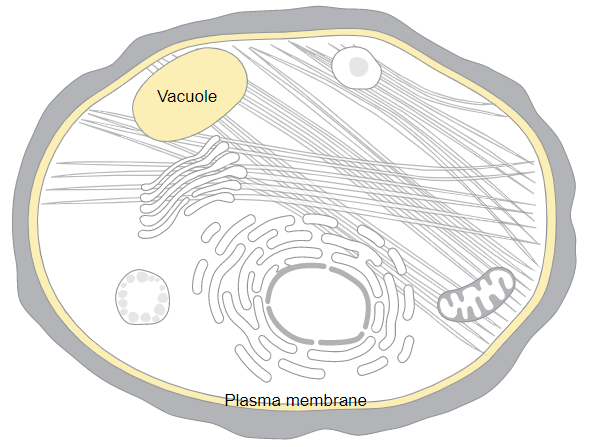
\includegraphics{subcell}
    \caption{苏氨酸蛋白激酶TOR1亚细胞定位图}
    \label{fig:subcell}
\end{figure}

\subsubsection{蛋白质拓扑相似性的邻边特征嵌入}

蛋白质在$PIN$中所处的拓扑环境也可以作为蛋白质相似性特征的计算方式。惭愧DPClus算法\cite{altaf-ul-amin_development_2006},本文将结点的公共邻居数作为拓扑相似性特征。具体计算方法如下:
\begin{equation}
    \label{equ:feat:topoCN}
    CN_{(P,Q)} = \left\lvert N_P\cap N_Q\right\rvert
\end{equation}
其中$P$,$Q$为相互作用的蛋白质,$N_P$和$N_Q$分别为两个蛋白质在$PIN$中的邻居。

\subsubsection{邻边特征嵌入汇总}

在数据预处理阶段,本文计算了$PIN$中所有蛋白质相互作用之间的相似性特征,其中包括蛋白质功能注释特征、结构域特征、亚细胞定位特征以及网络拓扑特征。$PIN$中每条相互作用边所具有的特征维度为12维,具体分布如表\ref{tab:PINedgeFeatNUms}所示:
\begin{table}[h]
    \centering
    \caption{$PIN$边特征维度分布}
    \label{tab:PINedgeFeatNUms}
    \begin{tabular}{C{3cm}C{3cm}C{3cm}C{3cm}}
        \toprule
        \textbf{功能注释特征} & \textbf{结构域特征} & \textbf{亚细胞定位特征} & \textbf{网络拓扑特征} \\
        \midrule
        2                     & 7                   & 2                       & 1                     \\
        \bottomrule
    \end{tabular}
\end{table}


\subsection{融合结点特征和邻边特征的蛋白质相互作用网络构建}
\label{subsection:featPPINetwork:addFeat}


\section{训练和待筛选复合物特征子图样本生成}
\label{section:featSubNetworkConstruct:allSample}

在$Feated-PIN$的基础上,按照复合物的对应结点抽取局部图$Feated-subGraph$,该局部图包含了复合物内部蛋白质之间的相互作用关系、相关性特征数据及部分蛋白质特征数据,因此可以将局部图作为后续复合物筛选模型的输入数据。

本文正样本由酵母菌标准复合物数据集CYC2008\cite{pu_up--date_2009}和MIPS\cite{pagel_mips_2005}构成,负样本为$PIN$上在一定限制条件下产生的随机子图。COACH算法\cite{leung_predicting_2009}作为在复合物预测方法中具有一定准确度和鲁棒性的方法,其产生的样本作为中间样本。


\subsection{正样本数据——基于已知蛋白质复合物融合}
\label{subsection:allSample:positiveSampleData}

本文融合了CYC2008和MIPS数据集,剔除了其中邻居相似性(公式\ref{equ:compComplexSim:NA})过高的部分,剩余的样本数为734。
在PPI网络中,可能存在部分结点缺失,为了保证标准复合物的准确性,在训练过程中我们舍弃具有缺失的标准复合物。具体数据为在Biogrid网络中,正样本个数为621个,在DIP网络中,正样本个数为371。

\subsection{中间样本数据——基于COACH算法}
\label{subsection:allSample:middleSampleData}

中间样本由无权COACH算法运行在目标网络中产生,需要对标准复合物和随机复合物具有一定的区分度,同时能对分类器识别复合物具有指导作用。一般情况下,通常复合物预测算法无法无法得到和标准集中的复合物完全相同的结果,在邻居相似性大于0.25时就认为复合物预测成功。

依据基于邻居相似性的分类标准,COACH生成的样本中有部分复合物预测成功,剩余的复合物预测失败,本文对分类模型的要求时可以区分这两类样本。在可区分该两类样本的情况下,模型对其他算法产生的结果进行筛选时,才可以正确的定位到其中预测成功的样本。因此本文将COACH生成的样本分为两类。
由于邻居相似性处于0.25附近时,样本可能具有较大的迷惑性,反而影响模型的正常训练,因此剔除相似性在0.25附近的部分样本。

本文对中间样本具体做如下处理:
\begin{enumerate}
    \item 计算各个样本和标准复合物的最高邻居相似性,得到0$\thicksim$1的分数;
    \item 剔除其中相似性分数高于0.8的样本,防止样本与标准集重合;
    \item 将相似性分数在0.4$\thicksim$1的样本作为A样本;
    \item 将相似性分数在0$\thicksim$0.2的样本作为B样本;
\end{enumerate}

经过上述处理,分别得到Biogrid网络和DIP网络运行COACH算法的中间样本数据集,其中Biogrid的A样本为192个、B样本为975个,DIP的A样本为179个、B样本为345个。

\subsection{负样本数据——基于权重动态随机密集子图生成}
\label{subsection:allSample:negtiveSampleData}


随机符合物是在互作网络中随机游走产生的随机图,结合标准样本和中间样本具有紧密型子图的特点,本文对随机游走算法做了一定限制。

首先按照图结点的权重选取初始结点,视作子图。对子图周围所有邻居结点设置权重,邻居结点与子图连接数越高,则该邻居结点权重越高。按照邻居结点权重加权随机抽取下一个结点,并将该结点加入子图,如此反复进行直至子图结点个数达到阈值。按照该种随机子图生成方法,子图趋向于密集连接。由于负样本在子图结构上和正样本相近,在进行分类任务时,可以避免模型学习简单的拓扑差异,迫使模型学习复合物内在的形成规律,达到主动学习的目的。图\ref{fig:diffrent-random-garphs}在DIP网络中采用不同随机算法得到的随机子图差异。

\begin{figure}[htbp]
    \centering
    \subcaptionbox{完全随机子图示意图1}{\label{fig:randomgraph:zitu:a}
        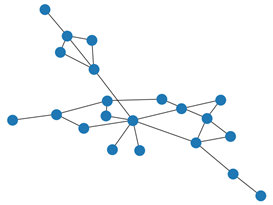
\includegraphics[width=5cm]{randomgraph-old-1}\hskip2cm}
    \subcaptionbox{完全随机子图示意图2}{\label{fig:randomgraph:zitu:b}
        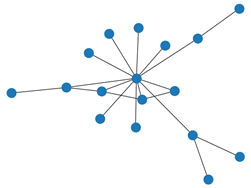
\includegraphics[width=5cm]{randomgraph-old-2}}
    \vskip0.5cm
    \subcaptionbox{限制性随机子图示意图1}{\label{fig:randomgraph:zitu:c}
        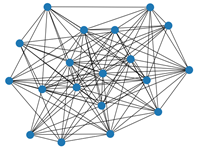
\includegraphics[width=5cm]{randomgraph-new-1}\hskip2cm}
    \subcaptionbox{限制性随机子图示意图2}{\label{fig:randomgraph:zitu:d}
        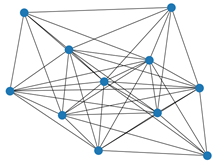
\includegraphics[width=5cm]{randomgraph-new-2}}
    \caption{不同随机算法获取的负样本差异图}
    \label{fig:diffrent-random-garphs}
\end{figure}


本文在网络中按照真实样本的结点数分布抽取负样本,负样本个数为标准样本和中间样本之和。

\subsection{待筛选样本数据——基于核心附属的蛋白质复合物预测算法}
\label{subsection:allSample:coreAttachSampleData}
\subsection{数据汇总与分析}
\label{subsection:allSample:summary}

最终产生的整体结果如下表所示:

\begin{table}[h]
    \centering
    \caption{数据集分布统计表}
    \label{tab:datasets:statistic}
    \begin{tabular}{C{3cm}C{2cm}C{3cm}C{3cm}C{2cm}}
        \toprule
        \textbf{网络} & \textbf{正样本数} & \textbf{中间样本数(A)} & \textbf{中间样本数(B)} & \textbf{负样本数} \\
        \midrule
        Krogan数据集  & 621               & 192                      & 975                      & 819               \\
        DIP数据集     & 371               & 179                      & 345                      & 764               \\
        \bottomrule
    \end{tabular}
\end{table}



\section{本章小结}
\label{section:FeatSubNetworkConstruct:summary}

\chapter{基于图卷积神经网络的复合物筛选模型}
\label{chapter:NodeConv}

本章介绍利用结点特征基于图卷积神经网络的复合物筛选模型,介绍了模型实现的细节和整体的模型实现流程。同时本章介绍了通用的相关的实验参数与指标。最后本章进行了相关实验并对实验结果进行了分析。

\section{引言}
\label{section:NodeConv:Put}

已有的基于监督学习的复合物预测算法,基本都是基于挖掘复合物子图的拓扑特征,比如图的密度、图的结点个数、平均度数等等,将图的所有拓扑特征置于一个向量中,构成一个$1\times N$的向量,用该向量代替子图,最后将向量用于训练分类模型。具体过程如图\ref{fig:entropy-classification}所示。

\begin{figure}[htbp]
    \centering
    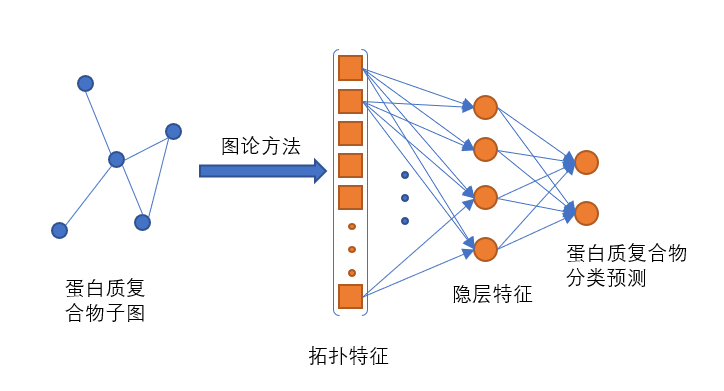
\includegraphics[width=12cm]{entropy-classification}
    \caption{基于图拓扑特征的蛋白质复合物分类模型}
    \label{fig:entropy-classification}
\end{figure}


但是蛋白质复合物中,有大部分复合物是小尺度复合物,其蛋白质个数小于5个。此类复合物的拓扑结构结构简单,提取的拓扑特征具有趋同性。随机的子图在结点数较少的情况下可能形成相同的拓扑特征,此时分类模型无法区分子图是否为真正的复合物。

蛋白质复合物网络是一个高维结构,可以通过挖掘蛋白质在网络中所处的位置和其周围相互作用关系挖掘蛋白质的潜在特征表示,将网络的高维数据转换为蛋白质的低维嵌入表示,成为每一个蛋白质初始的特征向量。

在不引入额外的生物学信息的情况下,本文提出了基于结点的全局拓扑特征的复合物局部子图分类模型。该模型仅使用网络的拓扑特征,利用图卷积神经网络在将拓扑信息与局部子图相互融合,最终得到局部子图的总体特征并做相应的分类与回归处理。

\section{基于图卷积神经网络的复合物筛选模型}
\label{section:NodeConv:detail}

\subsection{基于结点卷积单层更新}

本文在\ref{subsection:featPPINetwork:nodeFeatConstruct}部分简单介绍了图卷积神经网络。本节介绍在基于图卷积神经网络的复合物筛选模型中单一图卷积网络的计算方法。

在单一的卷积层中,结点特征的计算方法如下图所示。

\begin{figure}[htbp]
    \centering
    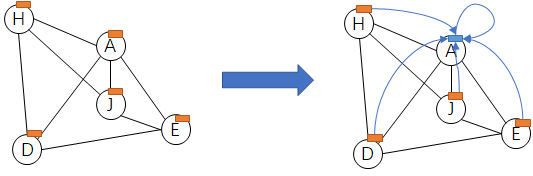
\includegraphics[width=10cm]{GCN/nodeupdate}
    \caption{结点更新过程中数据流程示意图}
    \label{fig:GCN/nodeupdate}
\end{figure}
如图中所示,结点A的特征将有结点$\{A,D,E,H,J\}$共同确定,图中左侧为未更新状态,右侧为更新结点特征过程中的数据流动。其具体过程可以表示为如下的公式。
\begin{equation}
    \label{equ:normalgcn}
    h_i^{(l+1)} = \sigma(b^{(l)} + \sum_{j\in\mathcal{N}(i)}\frac{1}{c_{ij}}h_j^{(l)}W^{(l)})
\end{equation}
其中$\mathcal{N}(i)$表示结点i的所有邻居,${c_{ij}}$表示结点i和结点j度乘积的平方根,其具体计算为$c_{ij} = \sqrt{|\mathcal{N}(i)|}\sqrt{|\mathcal{N}(j)|}$,$\sigma$表示激活函数,$b^{(l)}$表示卷积过程中的偏移值。

在模型中,偏移值设置为0,激活函数为Relu函数。而在卷积过程中,为了保持结点特征的连续性,每一个子图的结点均添加一条自环,从式中可以得出,添加自环之后,结点特征更新过程中会有一部分信息由自身提供。

上式为单个结点的更新过程,将子图中所有结点更新一轮之后即完成一层图卷积过程,图中结点特征从第l层更新到第l+1层。

\subsection{特征子图评价模型}
\label{subsection:NodeConv:flow}

下面从数据流的层面阐述从特征子图数据到样本评价数据的实现流程。基于全局特征的复合物分类模型总体结构如图\ref{fig:GCN/flow}所示。
\begin{figure}[htbp]
    \centering
    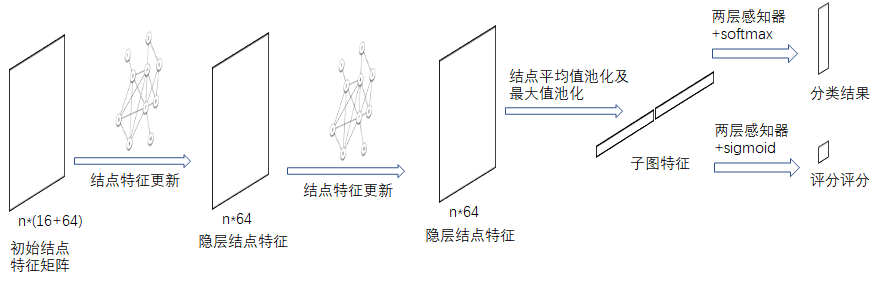
\includegraphics[width=14cm]{GCN/flow}
    \caption{基于图卷积神经网络的复合物筛选模型总体流程}
    \label{fig:GCN/flow}
\end{figure}
模型的初始输入特征结点特征,维度为80维,其中包括基于Deepwalk嵌入特征64维和GAE嵌入特征16维。
在初始特征之后加入了两层图卷积模型,图卷积模型如\ref{section:NodeConv:detail}所示,图卷积可以融合图中结点特征和拓扑结构对结点特征进行更新。图卷积过程中隐层维度设置为64维。两层图卷积之后,采用了对结点特征MaxPooling和MeanPooling的池化方法。两种池化方法的结果进行拼接之后,形成的128维的特征代表图整体特征,如图中1和2部分所示,1部分代表MaxPooling得到的64维特征,2部分代表通过MeanPooling得到的64维特征。

分类与评分部分,3和4即代表了两种Pool方法拼接之后的结果,作为代表子图的特征向量。
后续分别为两层感知器和softmax层得到图的分类预测,两层感知器和sigmoid层得到图的评分预测。而两项预测结果采用公式\ref{equ:loss}的损失函数统一起来。通过不断的优化损失函数,可以使得特征向量同时具备分类与评分特征。

分类指标和评分将作为蛋白质复合物的综合评价指标,具体计算方法如\ref{section:NodeConv:allExperienceDesign}中损失函数计算部分所示。

\subsection{筛选模型算法流程}

具体算法如下所示。

\begin{algorithm}[h]
    \caption{基于图卷积神经网络的复合物筛选模型} % 名称
    \label{alg::nodeconv}
    \begin{algorithmic}
        \Require
        $PIN$:Protein-Protein Interaction Network

        \Ensure
        $F_1$
        \State initial nodefeat=1, $F_0$;initial i=0;
        \Repeat
        \State compute hidden feat 1, $F_1=GCN(G,F_0)$;
        \State compute hidden feat 2, $F_2=GCN(G,F_1)$;
        \State compute hidden feat 3, $F_3=GCN(G,F_1)$;
        \State reconstruct graph, $A^{\prime}=Dec(F_3)$;
        \State compute loss, $L=MSELoss(A^{\prime},A)$;
        \State optimization, $Adam(L)$;
        \State i=i+1;
        \Until{$i=80$}
        \State extract node feats to $F$, $F$=$F_3$;
    \end{algorithmic}
\end{algorithm}

\section{实验参数与评估指标}
\label{section:NodeConv:allExperienceDesign}
本节介绍实验相关环境、实验通用超参数设置、相关优化器以及评估指标,该部分内容适用于本文所有复合物筛选模型的实验,后续章节中不做重复阐述。

\subsection{实验环境}
\label{subsection:allExperienceDesign:Environment}

本文的实验基于Linux系统Ubuntu16.04版本,处理器型号为Intel(R) Xeon(R) CPU E5-2680 v4 @ 2.40GHz,内存大小为128GB。本文代码基于Python编写,其中深度学习框架基于Pytorch,图神经网络框架基于DGL库\cite{wang_deep_2020}。

\subsection{实验参数}
\label{subsection:allExperienceDesign:nums}

由于训练数据的不平衡性,训练模型之前,数据进行了重采样处理,保持各分类训练样本相等。按照$8:2$的比率分割各分类样本,形成训练集和测试集。在分类模型的训练过程中,观察训练集和测试集的损失函数,根据早停策略得到未过拟合最佳模型。
由于各项特征数据存在不平衡性,部分数据如蛋白质长度等数值过大,本文将所有的特征数据进行了统一的归一化和标准化处理。

本文采用0.001的学习率,batch大小设置为32,隐层维度为128,模型使用了两层的GCN网络以及两层的分类器。
采用LeakyRelu作为激活函数和AdamOptimizer作为模型优化器。LeakyRelu激活函数如图\ref{fig:leakyrelu}所示。

\begin{figure}[htbp]
    \centering
    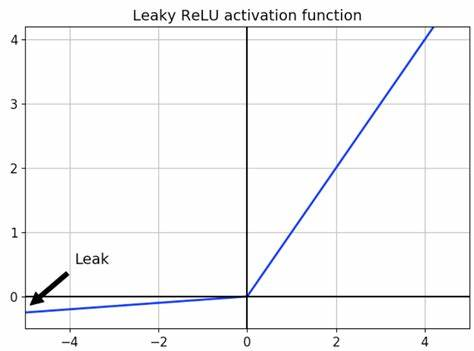
\includegraphics[width=5cm]{leakyrelu}
    \caption{Leaky-Relu 激活函数示意图}
    \label{fig:leakyrelu}
\end{figure}
LeakyRelu激活函数会保留所有为正值的数据,相较于Relu激活函数将所有输入的负值以0输出,LeakyRelu会保留一定的负值输出。


每一个训练复合物样本都具有复合物类别以及相似性评分两项数据,针对这两项属性,本文实验中分别设置了两项损失函数,使用交叉熵损失(Cross Entropy Loss)计算复合物类别分类损失,使用BCE损失(Binary Cross Entropy Loss)计算复合物得分回归损失。由于两项损失在数值上的差异,设置了相应的损失平衡系数。具体损失计算如下所示。
\begin{equation}
    \label{equ:loss}
    loss=CELoss(PL,TL)+\alpha \cdot BCELoss(PS,TS)
\end{equation}
其中,$PL$为预测类别,$TL$为真实类别,$PS$为预测评分,$TS$为真实评分,$\alpha$为损失平衡系数。

\subsection{评估指标}
\label{subsection:allExperienceDesign:metrix}

模型测试阶段,本文将复合物生成算法A在$PIN$网络中运行得到算法A预测的复合物$Complexes_A$,用复合物分类模型筛选所有预测结果,其中如果预测样本在筛选模型中被分类为真样本或者评分高于0.25时,预测样本即可通过筛选。最后所有通过筛选的复合物形成复合物集合$Complexes_A'$。最后使用F1值和PPV指标评估$Complexes_A$和$Complexes_A'$的复合物质量。
评价复合物预测结果的常用指标为精准率(precision)、召回率(recall)和F1值(F1-score)。预测复合物和标准复合物计算邻居相似性(NA-similarity)\ref{equ:compComplexSim:NA}。

按照一般性标准,邻居相似性大于0.25时,预测复合物和标准复合物具有匹配性,表示复合物预测成功。
精准率计算如公式\ref{equ:precision}所示。
其中$PC$为预测复合物集合,$M_{PC}$为预测复合物中具有匹配性的所有复合物集合。精准率表示预测复合物中,预测成功的样本所占比重,衡量预测结果的“查准率”。
召回率段计算如公式\ref{equ:recall}所示。
其中$BC$为标准复合物集合,$M_{BC}$为标准复合物中被预测复合物匹配的集合。召回率表示标准复合物中,能被预测复合物匹配的样本所占的比重,衡量预测结果的“查全率”。
F1值综合考虑查准率和查全率,计算如公式\ref{equ:f1}所示。
从定义看出,当查准率和查全率中有一项指标偏小时,F1值就会偏小。
\begin{equation}
    \label{equ:precision}
    precision=\frac{\left\lvert M_{PC}\right\rvert }{\left\lvert PC\right\rvert }
\end{equation}
\begin{equation}
    \label{equ:recall}
    recall=\frac{\left\lvert M_{BC}\right\rvert }{\left\lvert BC\right\rvert }
\end{equation}
\begin{equation}
    \label{equ:f1}
    f-score=\frac{2\times precision\times recall}{precision + recall }
\end{equation}

除此之外,研究者还提出了多种评价复合物预测质量的指标\cite{shi_protein_2011},包括Sn值、PPV值(Cluster-wise Positive Predictive Value)和Acc值等等。

Sn值具体计算方式图式\ref{equ:Sn}所示,
\begin{equation}
    \label{equ:Sn}
    S_n=\frac{\sum_{i = 1}^{n} \max_{j=1}^{m} t_{ij}}{\sum_{i = 1}^{n}n_i}
\end{equation}
其中${j| 1,2,\dots,m }$表示所有的预测复合物,${i| 1,2,\dots,n }$表示所有的标准复合物,$t_{ij}$表示两个复合物$i,j$之间共同蛋白质的数量,$n_i$表示真实复合物中蛋白质的个数。$S_n$值可以反应真实复合物中蛋白质分子被匹配到个数的平均值。

PPV值具体计算方式如式\ref{equ:PPV}所示,
\begin{equation}
    \label{equ:PPV}
    PPV=\frac{\sum_{j = 1}^{m} \max_{i=1}^{n} t_{ij}}{\sum_{i = 1}^{n} \sum_{j = 1}^{m}   t_{ij}}
\end{equation}
可以看出PPV值反应了预测的复合物的匹配程度,PPV值越高,表示预测复合物和标准复合物的平均重合度越高。

Acc值综合考虑了Sn值和PPV值的结果,能更全面的反应预测复合物集合的质量,其具体计算方法如式\ref{equ:Acc}所示。通常情况下,可以将Sn值、PPV值和Acc值的和作为综合的衡量指标\ref{equ:SPA}。
\begin{equation}
    \label{equ:Acc}
    Acc=\sqrt{S_n\times PPV}
\end{equation}

\begin{equation}
    \label{equ:SPA}
    SPA= Sn+PPV+Acc
\end{equation}

\section{实验设计及结果分析}
\label{section:NodeConv:experience}

本章提出了基于全局特征的复合物筛选模型,该模型使用蛋白质网络得到蛋白质编码,在复合物子图中使用GCN网络将蛋白质编码和子图拓扑结构进行融合。
该模型未引入额外的生物学信息,为了验证模型的有效性,本文进行了如下的对比试验。

第一个对比的模型是使用随机特征GCN图分类模型,子图GCN网络输入的结点特征为随机数据,通过该模型的对比验证全局特征的有效性。

第二个对比的模型是采用图论拓扑特征的分类模型\ref{fig:entropy-classification}。计算若干维度的图拓扑特征并进行标准化处理,作为子图特征的代表,用于后续多层感知器分类模型的输入。具体特征提取拓扑特征如表\ref{tab:datasets:statisticgraphfeat}所示。

\begin{table}[h]
    \centering
    \caption{图拓扑特征统计}
    \label{tab:datasets:statisticgraphfeat}
    \begin{tabular}{C{3cm}C{2cm}L{8cm}}
        \toprule
        \textbf{拓扑特征类型} & \textbf{维数} & \textbf{具体描述}                \\
        \midrule
        图总体特征            & 2             & 图结点数,图密度                 \\
        度分布特征            & 4             & 度数平均值、最大值、最小值、方差 \\
        聚类系数特征          & 3             & 聚类系数最大值、平均值、方差     \\
        其他特征              & 1             & 度同配型(degree assortativity) \\
        \bottomrule
    \end{tabular}
\end{table}

图\ref{fig:result/DIP/node}为在DIP网络中,随机结点特征模型、图论拓扑特征模型以及全局特征模型筛选之后结果的对比。
\begin{figure}[htbp]
    \centering
    \subcaptionbox{F1值对比}{\label{fig:result/DIP/F1/node}
        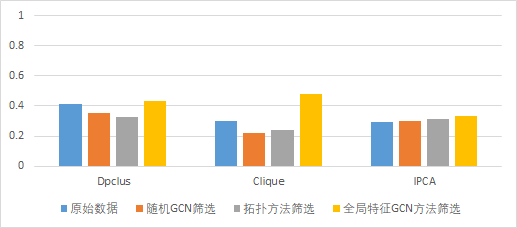
\includegraphics[width=10cm]{result/DIP/F1/node}}
    \vskip0.2cm
    \subcaptionbox{SPA值对比}{\label{fig:result/DIP/SPA/node}
        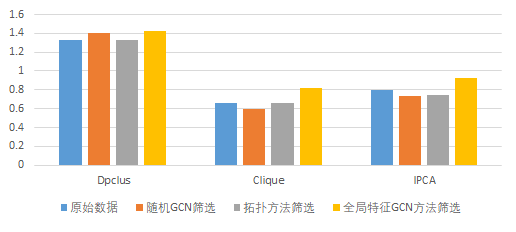
\includegraphics[width=10cm]{result/DIP/SPA/node}}
    \caption{DIP网络不同模型处理后结果对比}
    \label{fig:result/DIP/node}
\end{figure}
从图\ref{fig:result/DIP/node}可以看出在DIP网络中随机GCN筛选和基于拓扑GCN筛选可能导致F1值的降低和评价指标的降低,这个原因可能是简单模型在学习的过程中会直接学习直观的拓扑关系,导致分类的错误率较高,在筛选过程中会错误的剔除正样本,导致筛选之后样本质量反而降低。

全局特征的GCN筛选方法,在三个方法中均取得了最佳的F1值和SPA值,证明了全局特征的有效性。

图\ref{fig:result/Biogrid/node}为在Biogrid网络中,随机结点特征模型、图论拓扑特征模型以及全局特征模型筛选之后结果的对比。
\begin{figure}[htbp]
    \centering
    \subcaptionbox{F1值对比}{\label{fig:result/Biogrid/F1/node}
        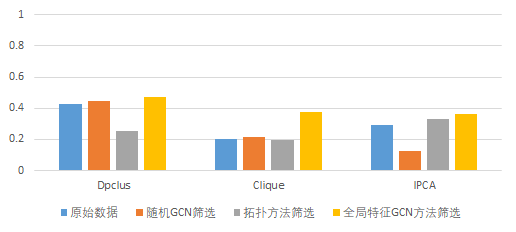
\includegraphics[width=10cm]{result/Biogrid/F1/node}}
    \vskip0.2cm
    \subcaptionbox{SPA值对比}{\label{fig:result/Biogrid/SPA/node}
        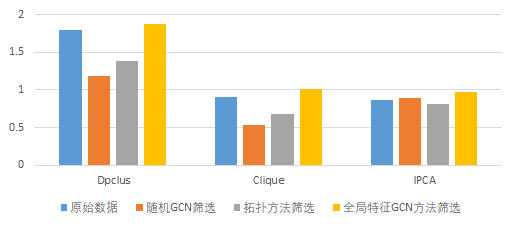
\includegraphics[width=10cm]{result/Biogrid/SPA/node}}
    \caption{Biogrid网络不同模型处理后结果对比}
    \label{fig:result/Biogrid/node}
\end{figure}

从图\ref{fig:result/Biogrid/node}中可以看出全局特征的GCN筛选对Clique算法的提升十分显著,原因是Clique算法是一种基于3-clique结构挖掘复合物的算法,该算法是一种基于密集连边发现复合物的算法,在Biogrid网络中,网络密度相较于DIP网络高了5.2,因此在Biogrid网络中,Clique算法会相应的产生更多的样本,从而为算法优化提供空间。

从上述结果可以得出。全局特征的GCN筛选方法对原始的样本数据的评价指标都有不同程度的提升。

图\ref{fig:result/DIP/node}和图\ref{fig:result/Biogrid/node}的数据如下所示。
\begin{table}[h]
    \centering
    \caption{DIP网络不同模型处理后结果对比数据}
    \begin{tabular}{C{2cm}C{2cm}C{2cm}C{2cm}C{2cm}}
        \toprule
        \textbf{F1值} & \textbf{原始数据} & \textbf{随机GCN筛选} & \textbf{拓扑方法筛选} & \textbf{全局特征GCN筛选} \\
        \midrule
        Dpclus算法    & 0.414             & 0.352                & 0.328                 & 0.434                    \\
        Clique算法    & 0.296             & 0.222                & 0.238                 & 0.477                    \\
        IPCA算法      & 0.291             & 0.300                & 0.310                 & 0.336                    \\
        \bottomrule
    \end{tabular}
    \begin{tabular}{C{2cm}C{2cm}C{2cm}C{2cm}C{2cm}}
        \toprule
        \textbf{SPA值} & \textbf{原始数据} & \textbf{随机GCN筛选} & \textbf{拓扑方法筛选} & \textbf{全局特征GCN筛选} \\
        \midrule
        Dpclus算法     & 1.333             & 1.340                & 1.330                 & 1.424                    \\
        Clique算法     & 0.658             & 0.596                & 0.656                 & 0.815                    \\
        IPCA算法       & 0.794             & 0.729                & 0.744                 & 0.922                    \\
        \bottomrule
    \end{tabular}
\end{table}

\begin{table}[h]
    \centering
    \caption{Biogrid网络不同模型处理后结果对比数据}
    \begin{tabular}{C{2cm}C{2cm}C{2cm}C{2cm}C{2cm}}
        \toprule
        \textbf{F1值} & \textbf{原始数据} & \textbf{随机GCN筛选} & \textbf{拓扑方法筛选} & \textbf{全局特征GCN筛选} \\
        \midrule
        Dpclus算法    & 0.425             & 0.444                & 0.254                 & 0.470                    \\
        Clique算法    & 0.202             & 0.216                & 0.196                 & 0.372                    \\
        IPCA算法      & 0.293             & 0.123                & 0.331                 & 0.365                    \\
        \bottomrule
    \end{tabular}
    \begin{tabular}{C{2cm}C{2cm}C{2cm}C{2cm}C{2cm}}
        \toprule
        \textbf{SPA值} & \textbf{原始数据} & \textbf{随机GCN筛选} & \textbf{拓扑方法筛选} & \textbf{全局特征GCN筛选} \\
        \midrule
        Dpclus算法    & 1.796             & 1.187                & 1.382                 & 1.871                    \\
        Clique算法    & 0.901             & 0.532                & 0.675                 & 1.009                    \\
        IPCA算法      & 0.859             & 0.886                & 0.810                 & 0.970                    \\
        \bottomrule
    \end{tabular}
\end{table}

\section{本章小结}
\label{section:NodeConv:summary}

本章基于拓扑结构出发,探讨了仅仅使用拓扑结构数据的基础上,复合物筛选模型可达到的效果提升。提出了利用GAE和Deepwalk特征基于图卷积神经网络的蛋白质复合物子图评分模型,阐述了单层卷积过程以及整体模型的结构。同时本章介绍了本文通用性的实验参数、基础以及评价指标。最后本章在基础模型,无特征模型上进行了实验,实验结果表明特征的有效性以及卷积融合结点特征后评价指标达到了最优结果。

\chapter{基于邻边卷积网络的复合物筛选模型}
\label{chapter:EdgeConv}

本章首先介绍了生物数据对复合物预测的重要性,介绍了生物数据在蛋白质相互作用网络中的邻边嵌入。同时介绍了基于邻边嵌入的相关图卷积算法,并提出了基于邻边卷积网络的复合物筛选模型。最后针对该模型进行了相关的对比实验并分析了实验结果。

\section{引言}
\label{section:EdgeConv:Put}

已有方法已经充分表明,在PPI网络中进行蛋白质复合物预测不仅仅是一个图论中的聚簇发现问题,更是一个信息融合问题。无论是加权网络方法、核心附属结构预测方法,都致力于最大程度的利用生物学信息进行辅助预测。

而已有的算法通常将生物学信息,包括GO功能注释、拓扑域、亚细胞定位等转换为蛋白质之间的相似性数据,即映射为邻边数据。已有的基于加权图的复合物预测算法是将邻边特征映射到固定的权重计算公式中,相较于基于无权图的算法,其预测复合物的质量有较好的提升,说明邻边数据在复合物预测领域具有一定的重要性。

然而,硬编码的过程只能将丰富的生物数据进行简单的映射,无法做到对生物数据的高维抽象。
目前该研究领域也尚未出现对邻边特征进行高维非线性抽象的算法。
基于以上前提,本文提出了利用生物特征基于邻边卷积网络的复合物局部子图分类模型。

\section{邻边卷积网络介绍}
\label{section:EdgeConv:intro}

邻边卷积网络\cite{wang_dynamic_2019}(EdgeBase Convolution)由点云学习领域提出,是一种基于邻边做特征转换以及特征聚合的方法。点云学习指的是使用计算机的方法学习与分析空间中独立数据点的集合,数据点的信息包括坐标、颜色、分类、强度值等等信息,数据点在空间中的集合状态即为点云。点云学习的任务是对点云数据做分割、物体识别等等。

在点云任务中,会与待更新结点i周围的K个最近邻居建立连边,基于连边做特征更新,然后所有的连边特征汇聚到一起作为结点的新特征。连边特征更新的过程中会考虑源点与汇点的信息流动,其具体的过程如图\ref{fig:EdgeConv/main}所示。
\begin{figure}[htbp]
    \centering
    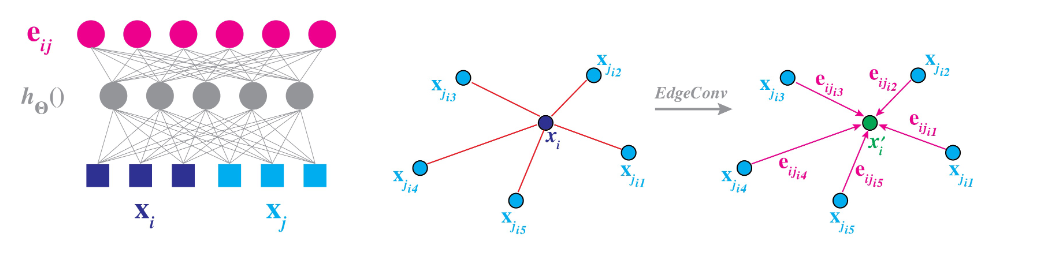
\includegraphics[width=14cm]{EdgeConv/main}
    \caption{基于邻边的图卷积神经网络更新示意图\cite{wang_dynamic_2019}}
    \label{fig:EdgeConv/main}
\end{figure}

对于结点i的更新,需要从结点i周围的5个邻居建立到结点i的邻边。对于其中某一条邻边$E_{j,i}$,其两个端点分别具有各自的特征,将特征拼接到一起,然后经过邻边卷积的多层感知器计算,即可得到邻边特征更新后的结果$e_{ij}$如图中左侧所示。
更新结点i周围所有的邻边特征,然后计算其和值,就形成了结点i更新之后的特征,如图\ref{fig:EdgeConv/main}中右侧所示。

\section{基于邻边卷积网络的复合物筛选模型}
\label{section:EdgeConv:detail}
本节分别介绍基于邻边卷积单层更新的具体实现,以及基于该单层更新方法构建的蛋白质复合物评价模型,最后介绍复合物筛选模型的总体实现流程。

\subsection{基于邻边卷积单层更新}

在通常的图卷积过程中,结点A的特征为周围所有结点的特征和自生特征决定,可以采取平均值的计算方法,如公式\ref{equ:NormalGCNNodeFlow}所示。
\begin{equation}
    \label{equ:NormalGCNNodeFlow}
    f_a=\delta (\frac{\sum_{i = 1}^{n}f_i+f_a}{n+1})
\end{equation}
其中$f_a$代表A结点的特征,$f_i$代表A结点所有邻居的特征,$\delta$为信息汇聚之后的特征更新函数。

在基于邻边卷积的复合物预测方法中,结点特征更新由其邻边共同决定。其具体计算过程如公式\ref{equ:EdgetoNodeFeat}所示。
\begin{equation}
    \label{equ:EdgetoNodeFeat}
    f_a=\delta (\frac{\sum_{i = 1}^{n}f_{ia}}{n})
\end{equation}
其中$f_{ia}$表示所有连接到A的邻边特征。其具体的汇聚过程如图\ref{fig:edge-feat-flow}所示,A结点汇聚周围所有邻边特征,包括$F_{BA}$、$F_{CA}$、$F_{DA}$以及$F_{EA}$。

\begin{figure}[htbp]
    \centering
    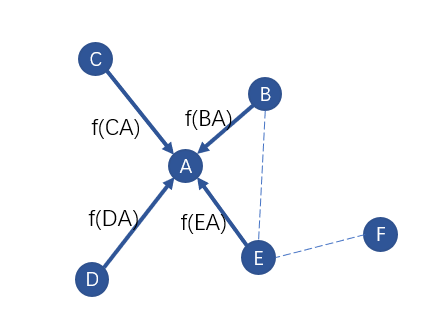
\includegraphics[width=7cm]{edge-feat-flow}
    \caption{边特征初始化结点特征示意图}
    \label{fig:edge-feat-flow}
\end{figure}

蛋白质生物数据是基于邻边的数据,因此在对复合物子图做图卷积的时候,基于生物特征的模型采用了基于edge的GCN模型\cite{wang_dynamic_2019},其具体的邻边更新方式如式\ref{equ:EdgeConv}所示。
\begin{equation}
    \label{equ:EdgeConv}
    h_i^{(l+1)} = \max_{j \in \mathcal{N}(i)} \mathrm{LeakyReLU}(
    \Theta \cdot (h_j^{(l)} - h_i^{(l)}) + \Phi \cdot h_i^{(l)})
\end{equation}
其中$h_i^{(l+1)}$表示第$l+1$层更新之后的结点数据,$h_j^{(l)} - h_i^{(l)}$表示从邻居结点到$i$结点的数据流,$h_i^{(l)}$为结点保留信息,$\Theta$和$\Phi$分别对应更新函数。$LeakyRelu$为激活函数。

每一轮基于edgeConv的卷积过程可以如下所示,首先是由结点更新邻边特征的过程,如图中上半部分所示,然后是用更新之后的邻边特征聚合物新的结点特征,如图中下半部分所示。

\begin{figure}[htbp]
    \centering
    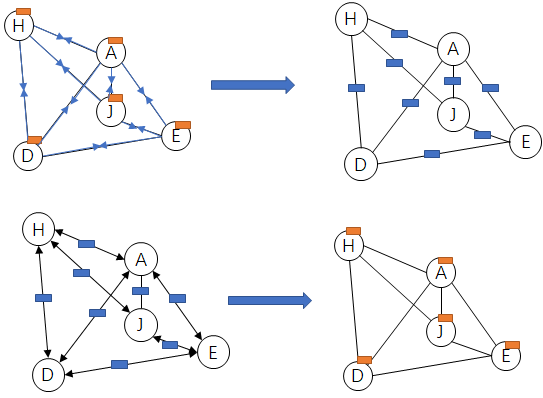
\includegraphics[width=10cm]{EdgeConv/edgeconv}
    \caption{总体EdgeConv图卷积过程示意图}
    \label{fig:EdgeConv/edgeconv}
\end{figure}

\subsection{特征子图评价模型}

本文处理了大量的生物学数据,包括蛋白质功能注释数据、结构域相互作用数据、亚细胞定位数据等,应用相关的生物领域的处理方法将生物学数据转换为可应用的特征数据,最终得到了11维度的特征数据。所有的特征都描述蛋白质相互作用,因此在图结构中,这些特征编码为图结构邻边的特征。
基于邻边卷积特征的复合物筛选模型总体流程如图\ref{fig:EdgeConv/flow}所示。

第一阶段如标号1所示,需要将初始的邻边特征以汇聚方法初始化结点特征,如图中上半部分所示。该汇聚方法为初始结点特征由其周围所有邻边特征的平均值替代。其具体的计算过程如公式\ref{equ:EdgetoNodeFeat}所示,其中激活函数为直接映射。其过程可被视为聚合阶段的基于边卷积神经网络过程,如图中\ref{fig:EdgeConv/edgeconv}下半部分所示。

第二阶段如标号2所示,需要基于邻边卷积将特征与拓扑结构融合,基于pool方法得到子图结构的特征表示,并基于子图特征做分类预测以及评分预测。其具体过程如图中下半部分所示。

模型使用了两层的基于邻边卷积的图神经网络,图卷积过程中隐层维度设置为64朴维。
两层图卷积之后,采用了对结点特征分别做最大值池化和平均值池化的方法,拼接到一起得到128维的子图特征。后续分别为两层感知器和softmax层得到图的分类预测,两层感知器和sigmoid层得到图的评分预测。


\begin{figure}[htbp]
    \centering
    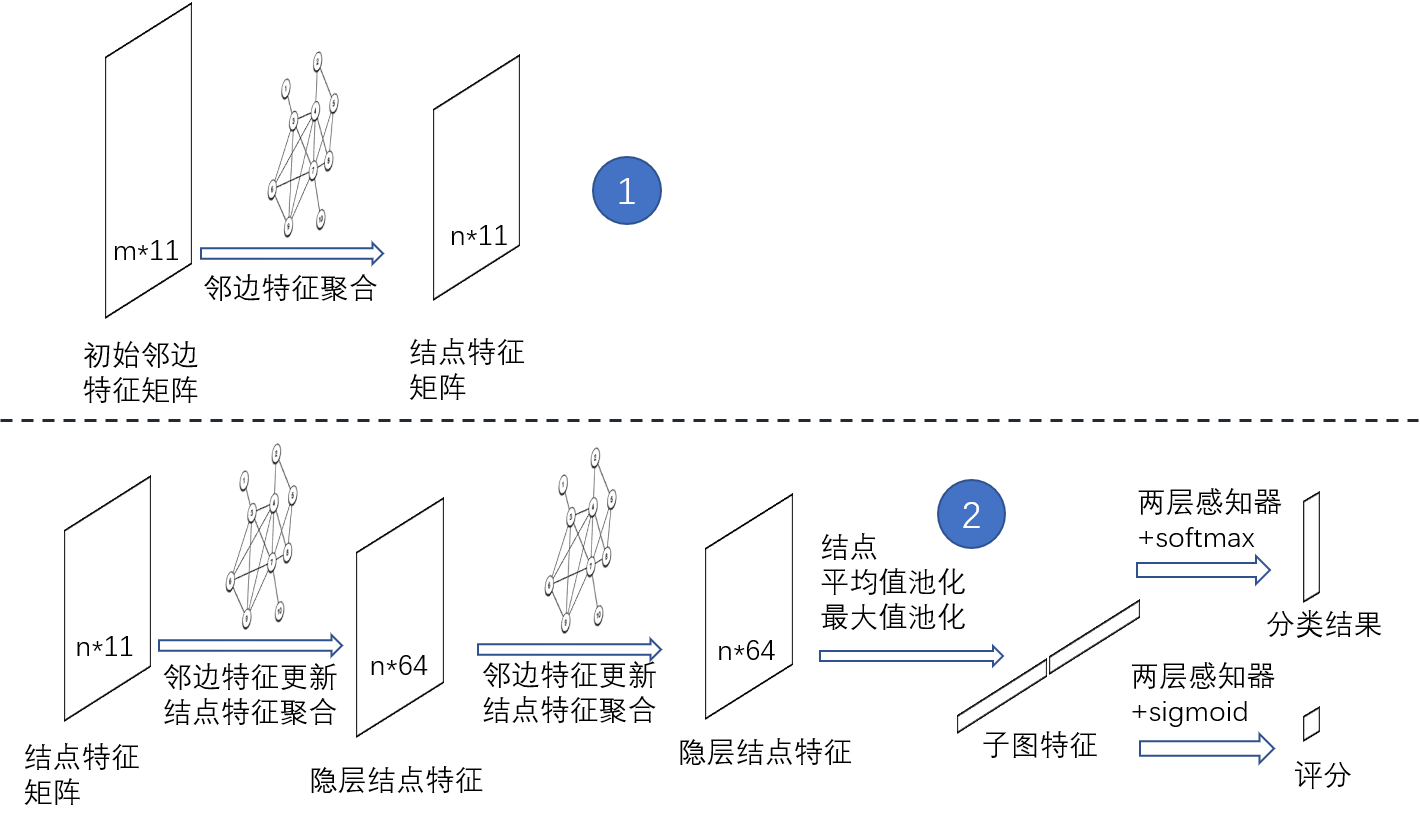
\includegraphics[width=16cm]{EdgeConv/flow}
    \caption{基于邻边卷积特征的复合物筛选模型总体流程}
    \label{fig:EdgeConv/flow}
\end{figure}

\subsection{筛选模型算法}
本节介绍基于邻边卷积的复合物筛选模型的具体算法,包括数据处理,模型训练,样本筛选与结果比对。
具体如算法\ref{alg:edgegcn-screen}所示。

\begin{algorithm}[h]
    \caption{Protein complex screening model based on edge convolution} % 名称
    \label{alg:edgegcn-screen}
    \begin{algorithmic}[1]
        \Require
        $Com_t$: train protein complexes;
        $Com_b$: protein complexes before screen;
        $Com_g$: golden bench protein complexes;
        $G$: protein-protein interaction network
        \Ensure
        $F1_a,F1_b/SPA_a,SPA_b$: predicted protein complexes F1/SPA metrix after and before screen;
        \State $n$:PIN node number;$m$:PIN edge number;$Com_a=None$;
        \State $F_{GO}\in \mathbb{R}^{m\times 2},F_{DDI}\in \mathbb{R}^{m\times 7},F_{Subcell}\in \mathbb{R}^{m\times 2},F_{Topo}\in \mathbb{R}^{m\times 1}$;
        \State $F_{E} \in \mathbb{R}^{m\times 12}=Concat(F_{GO},F_{DDI},F_{Subcell},F_{Topo})$;
        \State $Subs_t=Ext(G,F_{E},Com_t)$: feated subgraph extract algorithm;
        \For{i=0;i<epoch;i++}
        \For{$BSub_t \in Sub_t$} $loss=0$;
        \For{$Sub_t \in BSub_t$}
        \State $F_{N}^0 =MLP_m(Mean(Neighbor(F_{E}))), \in \mathbb{R}^{m\times 12}$;
        \State $F_{N}^1=EdgeConv(G,F_{N}^0), \in \mathbb{R}^{m\times 64}$
        \State $F_{N}^2=EdgeConv(G,F_{N}^1), \in \mathbb{R}^{m\times 64}$
        \State $F_t=Concat(MeanP(F_{N}^2),Maxp(F_{N}^2)), \in \mathbb{R}^{m\times 128}$;
        \State $PredC_t=MLP_C(F_t),\in \mathbb{R}^{1\times 4}$;$PredS_t=MLP_S(F_t),\in \mathbb{R}^{1}$;
        \State $loss+=\{CEL(PredC_t,LabelC_t)+\alpha \cdot BCEL(PredS_t,LabelS_t)\}$
        \EndFor; optimization $Adam(loss)$;
        \EndFor
        \EndFor
        \State $Subs_b=Ext(G,F_{E},Com_b)$: feated subgraph extract algorithm, see in \ref{section:featSubNetworkConstruct:allSample};
        \For{$Sub_b \in Subs_b$} $PredC_b=MLP_C(F_b)$;$PredS_b=MLP_S(F_b)$;
        \State $Com_a+=Complex(Sub_b)~if~PredC_b=positive|PredS_b>=0.25$;
        \EndFor
        \State $F1_a=F1(Com_a,Com_g),F1_b=F1(Com_b,Com_g)$;
        \State $SPA_a=SPA(Com_a,Com_g),SPA_b=SPA(Com_b,Com_g)$;
    \end{algorithmic}
\end{algorithm}
\section{实验设计及结果分析}
\label{section:EdgeConv:experience}

为了验证生物特征的添加对算法模型的提升,本文对比了在不添加生物数据,而使用相同的GCN结构的情况下,复合物分类模型对样本质量的提升程度。实验在DIP和Biogrid网络中分别运行了Dpclus、Clique和IPCA三个复合物生成算法。实验结果如下所示。
\begin{figure}[htbp]
    \centering
    \subcaptionbox{F1值对比}{\label{fig:result/DIP/F1/edge}
        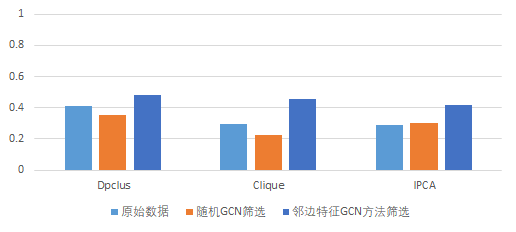
\includegraphics[width=10cm]{result/DIP/F1/edge}}
    \vskip0.2cm
    \subcaptionbox{SPA值对比}{\label{fig:result/DIP/SPA/edge}
        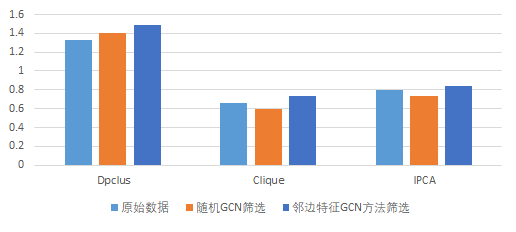
\includegraphics[width=10cm]{result/DIP/SPA/edge}}
    \caption{DIP网络不同模型处理后结果对比}
    \label{fig:result/DIP/edge}
\end{figure}

\subparagraph*{实验方案(一)} ~

图\ref{fig:result/DIP/edge}为在DIP网络中,随机特征模型和基于生物特征的模型筛选之后结果的对比。
从图中可以看出,添加了生物特征后,在DIP网络中复合物的生成质量得到了相应的提升,同样的由于CLique算法的特征,该算法的前后对比提升幅度最为明显。

\subparagraph*{实验方案(二)} ~

图\ref{fig:result/Biogrid/edge}为在Biogrid网络中,随机特征模型和基于生物特征的模型筛选之后结果的对比。
\begin{figure}[htbp]
    \centering
    \subcaptionbox{F1值对比}{\label{fig:result/Biogrid/F1/edge}
        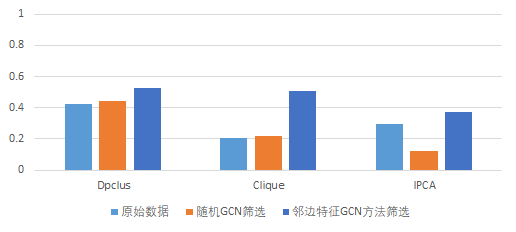
\includegraphics[width=10cm]{result/Biogrid/F1/edge}}
    \vskip0.2cm
    \subcaptionbox{SPA值对比}{\label{fig:result/Biogrid/SPA/edge}
        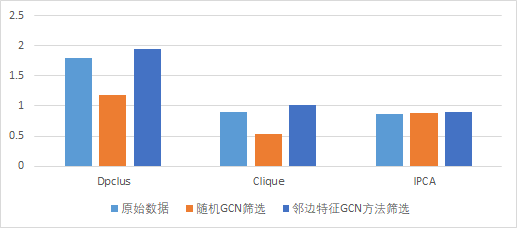
\includegraphics[width=10cm]{result/Biogrid/SPA/edge}}
    \caption{Biogrid网络不同模型处理后结果对比}
    \label{fig:result/Biogrid/edge}
\end{figure}
从图\ref{fig:result/Biogrid/edge}中可以看出添加了生物特征后,Biogrid网络相应样本的F1值均有较为明显的提升,而Clique算法的样本提升最为明显。综合评价指标SPA值也具有一定的提升。

图\ref{fig:result/DIP/edge}和图\ref{fig:result/Biogrid/edge}的数据如下所示。
\begin{table}[h]
    \centering
    \caption{DIP网络不同模型处理后结果对比数据}
    \begin{tabular}{C{2cm}C{2cm}C{2cm}C{2cm}}
        \toprule
        \textbf{F1值} & \textbf{原始数据} & \textbf{随机GCN筛选} &\textbf{邻边特征GCN筛选} \\
        \midrule
        Dpclus算法    & 0.414             & 0.352                & 0.484                                 \\
        Clique算法    & 0.296             & 0.222                & 0.453                              \\
        IPCA算法      & 0.291             & 0.300                & 0.420                               \\
        \bottomrule
    \end{tabular}
    \begin{tabular}{C{2cm}C{2cm}C{2cm}C{2cm}}
        \toprule
        \textbf{SPA值} & \textbf{原始数据} & \textbf{随机GCN筛选} & \textbf{邻边特征GCN筛选} \\
        \midrule
        Dpclus算法     & 1.333             & 1.340                & 1.490                                    \\
        Clique算法     & 0.658             & 0.596                & 0.731                                  \\
        IPCA算法       & 0.794             & 0.729                & 0.838                               \\
        \bottomrule
    \end{tabular}
\end{table}

\begin{table}[h]
    \centering
    \caption{Biogrid网络不同模型处理后结果对比数据}
    \begin{tabular}{C{2cm}C{2cm}C{2cm}C{2cm}}
        \toprule
        \textbf{F1值} & \textbf{原始数据} & \textbf{随机GCN筛选} &\textbf{邻边特征GCN筛选} \\
        \midrule
        Dpclus算法    & 0.425             & 0.445                & 0.529                                 \\
        Clique算法    & 0.203             & 0.216                & 0.510                              \\
        IPCA算法      & 0.294             & 0.122                & 0.373                               \\
        \bottomrule
    \end{tabular}
    \begin{tabular}{C{2cm}C{2cm}C{2cm}C{2cm}}
        \toprule
        \textbf{SPA值} & \textbf{原始数据} & \textbf{随机GCN筛选} & \textbf{邻边特征GCN筛选} \\
        \midrule
        Dpclus算法     & 1.796             & 1.119                & 1.950                                    \\
        Clique算法     & 0.901             & 0.532                & 1.011                                  \\
        IPCA算法       & 0.859             & 0.886                & 0.891                               \\
        \bottomrule
    \end{tabular}
\end{table}


\section{本章小结}
\label{section:EdgeConv:summary}

本章基于特征子图中的邻边相似性出发,探讨了仅仅使用生物特征转换为的邻边数据的基础上,复合物筛选模型可达到的效果提升。提出了使用基于邻边卷积的图神经网络方法以及相应的模型,阐述了邻边特征如何初始化结点特征,以及EdgeConv的信息流更新过程。最后本章对比了基础的无特征EdgeConv模型,并进行了实验,实验结果表明了生物特征的有效性以及邻边卷积能较好的处理生物相似性数据。
\chapter{基于消息传递网络的复合物筛选模型}
\label{chapter:MPNN}
\section{引言}
\label{section:MPNN:Put}

模型\ref{section:NodeConv:Put}和模型\ref{section:EdgeConv:intro}分别是结点嵌入和邻边嵌入模型,蛋白质复合物的形成和蛋白质特征以及蛋白质互作特征均具有相关性。
无论普通的GCN模型还是EdgeConv模型,均只能直接基于结点特征进行卷积运算,或者邻边特征转换为结点特征之后再进行图卷积运算,这个过程将邻边特征均匀的分配给了其相邻的结点,在模型训练过程邻边作为独立的计算元素依旧缺乏针对邻边本身的更新。这种情形下,邻边特征只能作为结点特征的补充,无法与复合物互作网络动态的结合起来。

为了将邻边特征与结点特征整合到模型的动态参数更新中,本节基于消息传递网络(Message Passing Neural Network,简称MPNN)提出蛋白质复合物特征融合模型,同时处理蛋白质复合物子图中的结点数据和邻边数据,将生物数据、全局拓扑特征以及局部拓扑特征动态的融合起来。
\section{消息传递网络介绍}
\label{section:MPNN:intro}

MPNN网络是一种基于消息传递的图结构学习框架。不同于图卷积模型必须将特征绑定到结点,MPNN将图结构的特征当成消息,特征在结构中的流动被视为消息的传递。在此框架下,图卷积神经网络可以被当作MPNN的特例,是只传递结点消息的MPNN网络。


MPNN网络的具体实现如式\ref{equ:MPNNPassing}所示。

\begin{equation}
    \label{equ:MPNNPassing}
    m_v^{t+1} = \sum_{w \in N_{(v)}}M_t(h_v^t,h_w^t,e_{vw}^t)
\end{equation}
\begin{equation}
    \label{equ:MPNNReadout}
    h_v^{t+1} = U_t(h_v^t,m_v^{t+1})
\end{equation}
其中$N_{(v)}$表示图中结点$v$的邻居,$t$为时间步。公式\ref{equ:MPNNPassing}表示消息传递阶段(Message Passing),$M_t$表示消息传递的更新函数,代表结点w向结点v传递消息的过程中,其传递的消息$h_v^t,h_w^t,e_{vw}$的更新方式。公式\ref{equ:MPNNReadout}表示更新阶段,$U_t$表示更新阶段的函数,代表结点v汇总所有周围消息后的数据更新方式。


\section{基于消息传递网络的复合物筛选模型}
\label{section:MPNN:detail}

基于消息传递网络的复合物筛选模型是基于MPNN网络的改进。
为了使得结点特征和邻边特征具有融合的能力,蛋白质复合物特征融合模型中采用了结点更新邻边,邻边更新结点的方式。在每一层的MPNN过程中,结点t时刻特征更新为邻边t+1时刻特征、邻边t特征更新为结点t+1时刻特征。结点特征的更新具体方法如下所示,其中$Linear$为一层感知器。
\begin{equation}
    \label{equ:MineMPNNPassing}
    m_v^{t+1} = \sum_{w \in N_{(v)}}Linear^t(e_{vw}^t)
\end{equation}

\begin{equation}
    \label{equ:MineMPNNReadout}
    h_v^{t+1} = Max(h_v^t,m_v^{t+1})
\end{equation}
从式中可以看出,结点的特征更新来源分为两部分,其一为汇聚所有邻边的特征$e_{vw}^t$,同时为了保留一部分结点中具有关键性的原始特征,其更新方式采用了maxpool。邻边特征的具体更新方法如下所示。
\begin{equation}
    \label{equ:MineMPNNedge}
    e_{vw}^{t+1} = Max(e_{vw}^t,Linear_0^t(m_w^{l} - m_v^{l}) + Linear_1^t m_v^{l})
\end{equation}
从式中得出,类似于结点更新模型,邻边的特征更新也可以分为两部分,最后同样采用了maxpool的方式保留关键邻边特征。邻边特征的更新方式综合考虑了源点到汇点的特征流动部分$m_w^{l} - m_v^{l}$以及汇点的特征保留部分$m_v^{l}$。


最后融合模型同样考虑了复合物子图的整体拓扑特征,为通过图论计算的总体拓扑结构数据,作为不可学习的特征与MPNN读出的特征拼接到一起,作为最终的图特征输出。总体拓扑特征计算参考\cite{yu_predicting_2014}。

\section{算法具体实现与流程}
\label{section:MPNN:flow}

子图数据保留GO注释特征、拓扑域特征以及亚细胞定位特征等邻边特征,保留Deepwalk特征、GAE特征等结点特征。形成兼具结点和邻边特征的复合物特征子图数据,其中结点特征维度为82维,邻边特征维度维12维。

\begin{figure}[htbp]
    \centering
    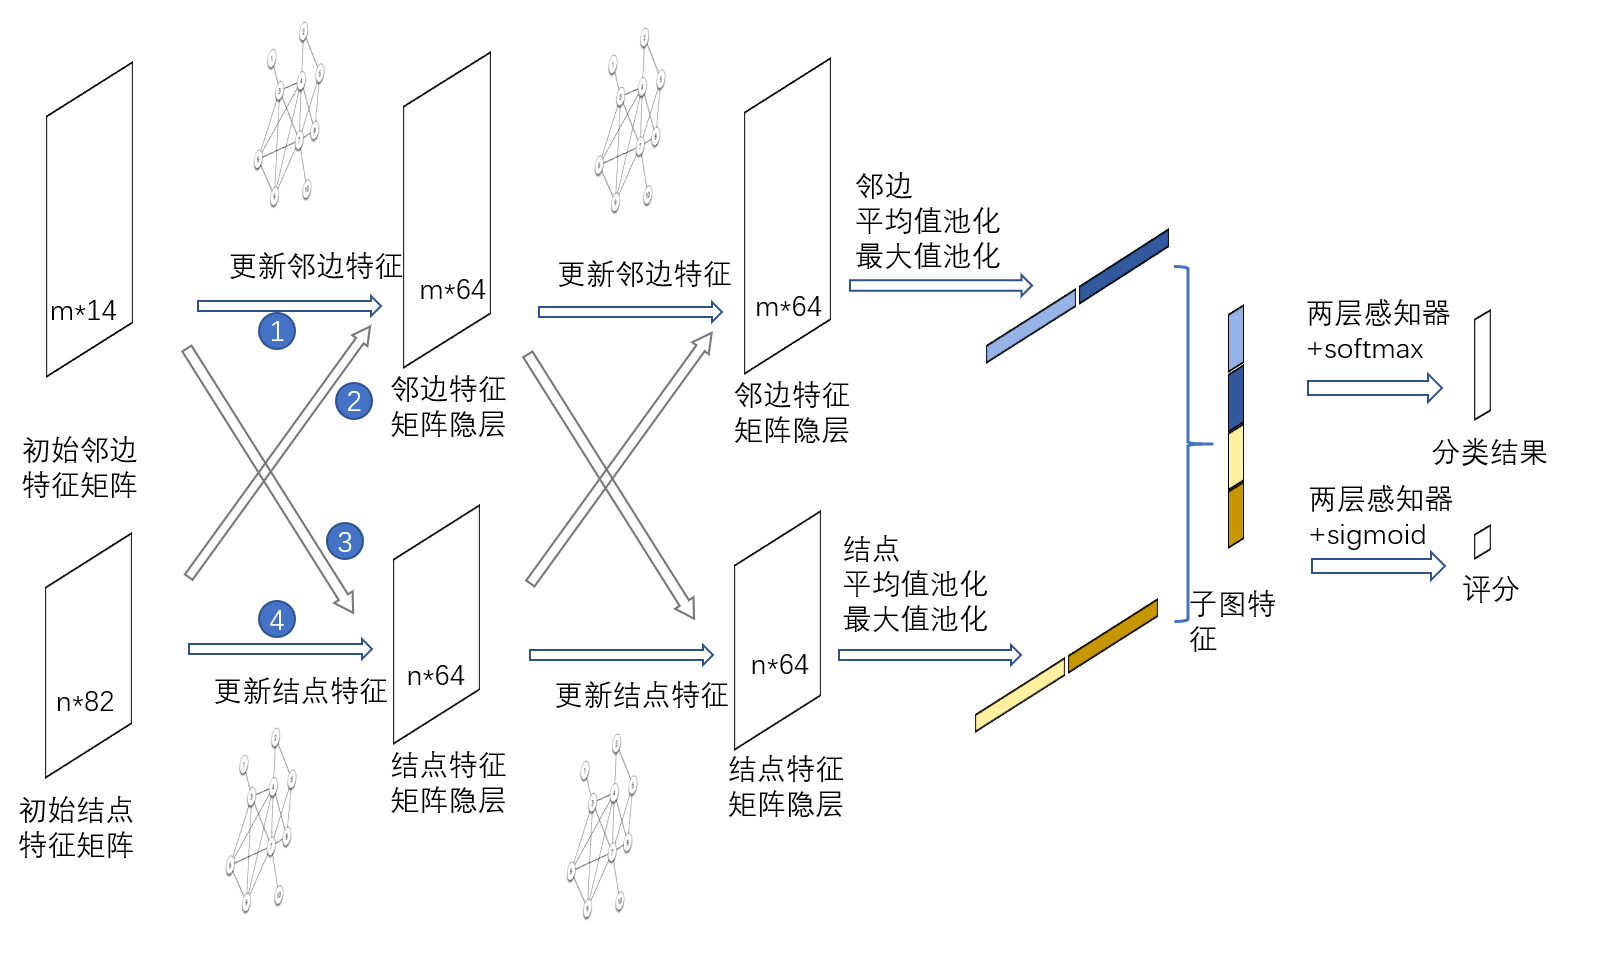
\includegraphics[width=14cm]{MPNN/flow}
    \caption{基于特征融合的分类模型总体流程}
    \label{fig:MPNN/flow}
\end{figure}

在模型中,添加了两层结点和邻边同时更新的MPNN网络,如图\ref{fig:MPNN/flow}所示。每一层MPNN网络中,结点特征更新由结点以及结点周围邻边特征共同确定,如示意图中的结点特征矩阵隐层的数据流所示,其具体的计算方法如公式\ref{equ:MineMPNNReadout}所示。邻边特征更新由邻边以及邻边两侧端点的结点特征共同确定,如示意图中的邻边特征矩阵隐层的数据流所示,其具体的计算方法如公式\ref{equ:MineMPNNedge}所示。

消息传递过程中隐层维度设置为64维,两层消息传递之后,采用了对结点特征Maxpool和MeanPool的池化方法以及对邻边Maxpool和MeanPool的池化方法。一共可以得出四个池化结果,对结果进行拼接之后,形成的256维的特征代表图整体特征。后续分别为两层感知器和softmax层得到图的分类预测,两层感知器和sigmoid层得到图的评分预测。

\section{实验设计及结果分析}
\label{section:MPNN:experience}
为了验证基于消息传递网络的模型的提升,本文对比了前两章分别设计的基于图卷积神经网络的复合物筛选模型和基于邻边卷积网络的复合物筛选模型。

基于图卷积神经网络的复合物筛选模型是基于研究蛋白质相互作用网络的拓扑结构展开,利用了结点的拓扑特征并基于结点的图卷积神经网络对拓扑特征进行融合,一定程度上体现了$PIN$网络中结点嵌入对复合物预测的作用,证实了复合物中蛋白质在互作网络中相关性对复合物的形成具有一定的影响。

基于邻边卷积网络的复合物筛选模型是基于研究蛋白质之间相似性特征展开,利用了邻边的相似性特征并基于邻边卷积对数据进行融合。生物的相似性数据对复合物预测以及复合物分类具有较明显的提升。

消息传递模型致力于向PIN网络全局特征以及生物特征融合到一起,分别以结点和邻边的形式嵌入到复合物子图中。相较于单独利用其中一方面的模型具有更好的预测能力。为了验证模型的有效性,本章进行了如下的实现。

实验在DIP和Biogrid网络中分别运行了Dpclus、Clique和IPCA三个复合物生成算法。实验结果如下所示。

图\ref{fig:result/DIP/fusion}为在DIP网络中,基于结点的全局特征模型、基于邻边的生物特征模型以及特征融合模型筛选之后结果的对比。
\begin{figure}[htbp]
    \centering
    \subcaptionbox{F1值对比}{\label{fig:result/DIP/F1/fusion}
        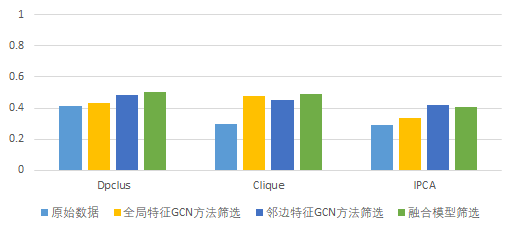
\includegraphics[width=10cm]{result/DIP/F1/fusion}}
    \vskip0.2cm
    \subcaptionbox{SPA值对比}{\label{fig:result/DIP/SPA/fusion}
        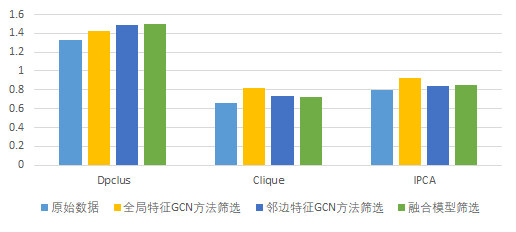
\includegraphics[width=10cm]{result/DIP/SPA/fusion}}
    \caption{DIP网络不同模型处理后结果对比}
    \label{fig:result/DIP/fusion}
\end{figure}

从图中可以看出,在DIP网络中,MPNN融合模型在F1的结果中取得了较大的提升,在Dpclus和Clique的数据样本中均得到了最优结果。

图\ref{fig:result/Biogrid/fusion}为在Biogrid网络中,基于结点的全局特征模型、基于邻边的生物特征模型以及特征融合模型筛选之后结果的对比。
\begin{figure}[htbp]
    \centering
    \subcaptionbox{F1值对比}{\label{fig:result/Biogrid/F1/fusion}
        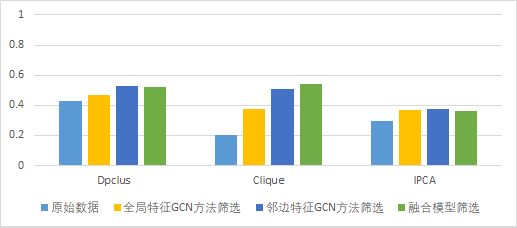
\includegraphics[width=10cm]{result/Biogrid/F1/fusion}}
    \vskip0.2cm
    \subcaptionbox{SPA值对比}{\label{fig:result/Biogrid/SPA/fusion}
        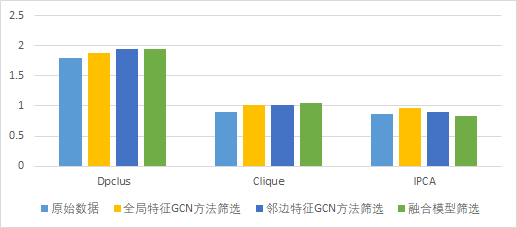
\includegraphics[width=10cm]{result/Biogrid/SPA/fusion}}
    \caption{Biogrid网络不同模型处理后结果对比}
    \label{fig:result/Biogrid/fusion}
\end{figure}
从图中可以看出,在Clique样本集上,其综合评价指标和F1值均达到了最优结果。而在Dpclus的样本集中,综合评价指标也得到了最优结果。


\section{本章小结}
\label{section:MPNN:summary}

本章基于特征融合出发,探讨了融合$PIN$全局特征以及生物相似性特征的情况下,模型设计以及进行了相关的实验。
在特征子图具有GAE和Deepwalk特征等结点特征、多种蛋白质相似性嵌入邻居特征的情况下,本章提出了改进的MPNN更新方法。提出了结点与邻边交替融合更新的模型。最后本章对比了利用结点特征的基于图卷积的模型,利用相似性特征的基于邻边卷积的模型,实验结果表明融合方法对于数据集中的结果具有一定的提升效果。
\chapter{结论与展望}
\label{chapter:SummaryAndForward}

\section{总结}
\label{section:allsummary}

生物学上蛋白质复合物的发现与研究对细胞组成、药物发现等研究至关重要。已有的蛋白质复合物预测方法主要思路是将蛋白质之间广泛的相互作用抽象成图结构,蛋白质复合物抽象为图结构中的局部结构,此时蛋白质复合物预测问题转换为了图结构的局部子图的发现问题。
然而这些方法通常聚焦于网络中挖掘子图的部分,将复合物预测当成加权或无权网络的密集子图发现问题,缺少对挖掘出的子图做评价的部分。

针对该问题,本文填补了蛋白质复合物的预测到对预测结果的评价之间存在的改进空间。
本文基于预测后复合物样本的评价与筛选模型研究(简称后筛选)设计可行且有效的模型框架,基于多种图卷积神经网络及其变种实现了复合物特征子图的评分模型。

本文第一章介绍了主流的蛋白质复合物预测算法,并根据存在的问题提出了可改进的空间。对研究背景、研究意义以及本文的主体研究流程做了相关介绍。
介绍了筛选模型的总体框架结构。
第二章阐述了具有结点特征和邻边特征的蛋白质相互作用网络的构建方法,包括GAE和Deepwalk的结点特征嵌入、以及多种基于蛋白质相似性计算的邻边嵌入方法;后续阐述了如何从特征相互作用网络中提取蛋白质复合物子图,以及训练子图样本、待筛选子图样本的生成方法。
第三章从拓扑特征入手,提出了利用结点的拓扑特征并基于结点的图卷积神经网络的复合物筛选模型,挖掘$PIN$网络中结点嵌入对复合物预测的作用。同时提出了本文算法框架中的参数细节,评价指标等等。后续进行了实验并验证模型的有效性。
第四章从特征子图中的邻边相似性出发,探讨了使用生物特征转换为的邻边数据的基础上,复合物筛选模型可达到的效果提升。提出了使用基于邻边卷积的图神经网络方法以及相应的模型,阐述了邻边特征如何初始化结点特征,以及EdgeConv的信息流更新过程。后续进行了相关对比实验并验证模型的有效性。
第五章在融合$PIN$全局特征以及生物相似性特征的情况下,提出了基于消息传递网络的复合物筛选模型。
特征子图具有GAE和Deepwalk特征等结点特征、多种蛋白质相似性嵌入邻居特征,提出了改进的MPNN更新方法,实现了结点与邻边交替融合更新的模型。最后对比了利用结点特征的基于图卷积的模型,利用相似性特征的基于邻边卷积的模型,并进行实验验证。

本文的研究成果如下:

1)构建融合结点特征和邻边特征的蛋白质相互作用网络。通过生物学上的多种特征提取方法,以及GAE、Deepwalk等网络嵌入方法,本文得到了兼具结点特征和邻边特征的$PIN$网络结构。

2)复合物子图数据集构建。基于邻居相似性融合多个标准集构建了正样本数据集;基于COACH算法的结果构建中间样本数据集;提出了改进的随机算法构建负样本数据集。在特征$PIN$中抽取特征子图作为训练样本。该样本集可供后续的复合物分类以及预测算法使用。

3)复合物分类模型研究。提出了蛋白质复合物评分模型并提出了基于提升已有方法预测质量的研究方法。在具有特征网络的前提下,本文研究了多种融合特征的复合物分类模型,提出了针对结点特征的图卷积模型、针对邻居特征的EdgeConv模型以及实现特征融合的消息传递网络模型。
本文首次将图分类模型引入了蛋白质复合物评价中,通过大量的实验验证了$PIN$网络中结点嵌入的有效性,生物数据作为邻边特征的有效性,以及融合方法的有效性。



\section{展望}
\label{section:forward}

本文提出了特征蛋白质互作网络构建,复合物特征样本集集以蛋白质复合物的评分模型。在此基础上,还有一部分研究可以进一步展开。

1)将蛋白质复合物评分模型作为复合物评价函数,利用强化学习的方法在蛋白质相互作用网络中挖掘蛋白质复合物。

2)本文使用的池化方法是基于平均池化和最大值池化,然而这种全局性质的池化方法可能丢失一部分蛋白质复合物子图的结构信息,后续可以考虑基于Graph Pool为基础的分层池化模型,以进一步在复合物特征表示上提升其拓扑表达能力。


% 参考文献
\printTJbibliography

\begin{acknowledgement}
    衷心感谢导师 xxx 教授和物理系 xxx 副教授对本人的精心指导。他们的言传身教将使
我终生受益。

在美国麻省理工学院化学系进行九个月的合作研究期间,承蒙 xxx 教授热心指导与帮助,不
胜感激。感谢 xx 实验室主任 xx 教授,以及实验室全体老师和同学们的热情帮助和支
持!本课题承蒙国家自然科学基金资助,特此致谢。

感谢 \tongjithesis{},它的存在让我的论文写作轻松自在了许多,让我的论文格式规整漂亮了
许多。
\end{acknowledgement}


\end{document}
